% ****** Start of file apssamp.tex ******
%
%   This file is part of the APS files in the REVTeX 4.2 distribution.
%   Version 4.2a of REVTeX, December 2014
%
%   Copyright (c) 2014 The American Physical Society.
%
%   See the REVTeX 4 README file for restrictions and more information.
%
% TeX'ing this file requires that you have AMS-LaTeX 2.0 installed
% as well as the rest of the prerequisites for REVTeX 4.2
%
% See the REVTeX 4 README file
% It also requires running BibTeX. The commands are as follows:
%
%  1)  latex apssamp.tex
%  2)  bibtex apssamp
%  3)  latex apssamp.tex
%  4)  latex apssamp.tex
%
\documentclass[%
 reprint,
superscriptaddress,
%groupedaddress,
%unsortedaddress,
%runinaddress,
%frontmatterverbose, 
%preprint,
%preprintnumbers,
%nofootinbib,
%nobibnotes,
%bibnotes,
 amsmath,amssymb,
 prl,
 %aps,
%pra,
%prb,
%rmp,
%prstab,
%prstper,
%floatfix,
]{revtex4-2}
\usepackage{centernot}
\usepackage{graphicx}% Include figure files
\usepackage{dcolumn}% Align table columns on decimal point
\usepackage{bm}% bold math
%\usepackage{hyperref}% add hypertext capabilities
%\usepackage[mathlines]{lineno}% Enable numbering of text and display math
%\linenumbers\relax % Commence numbering lines
\usepackage[dvipsnames]{xcolor}
%\usepackage[showframe,%Uncomment any one of the following lines to test 
%%scale=0.7, marginratio={1:1, 2:3}, ignoreall,% default settings
%%text={7in,10in},centering,
%%margin=1.5in,
%%total={6.5in,8.75in}, top=1.2in, left=0.9in, includefoot,
%%height=10in,a5paper,hmargin={3cm,0.8in},
%]{geometry}

\newcommand{\re}{\color{red}} %  for red comments, use 
\begin{document}

%\preprint{APS/123-QED}

\title{Theory for Adaptive Systems: Collective Robustness of Genotype-Phenotype Evolution}
%Robustness  in evolutionary theory with genotype-phenotype mapping --NEED TO BE REVISED}% Force line breaks with \\
%\thanks{A footnote to the article title}%

\author{Tuan Minh Pham}
\affiliation{The Niels Bohr Institute, University of Copenhagen,
Blegdamsvej 17, Copenhagen, 2100-DK, Denmark
}



\author{Kunihiko Kaneko}
\email{email: kaneko@complex.c.u-tokyo.ac.jp}
\affiliation{The Niels Bohr Institute, University of Copenhagen,
Blegdamsvej 17, Copenhagen, 2100-DK, Denmark
}
\date{\today}% It is always \today, today,
             %  but any date may be explicitly specified

\begin{abstract}
 The investigation of mutually coupled dynamics, involving many degrees of freedom on two separated  timescales, one for fast changes of state variables  and another for the slow adaptation of  parameters controlling  the former's dynamics is crucial for understanding biological evolution and learning.  We develop a general theory for such dynamics by extending  dynamical mean field theory. We then apply our  framework  to biological systems whose fate is determined by
the evolution of 
genotype-phenotype relationship. % . %Evolutionary theory for  such relation   needs to  encapsulate both   genetic variations and phenotypic variances by noise, rather than describing solely an uphill motion on a fitness-landscape in the space of genotypes. 
Here %through  genotypic mutations and  phenotype-based selection, 
phenotypic evolution is shaped by stochastic gene-expression fast dynamics and is coupled to  selection-based slow changes of genotypes encoding the network of gene regulations. We find   \emph{dynamically robust patterns} of phenotypes can be achieved  under an intermediate level of external noise  where  the genotype-phenotype relation evolves in such a way that results in intrinsic out-of-equilibrium fluctuations of phenotypes even in the absence of that noise. %a correlation between  robustnesses of phenotypes to noise and   to genetic mutations. %, as a result of replica symmetry.We also find a trade-off between maintaining a high fitness level of phenotype and acquiring a robust pattern of genes as well as the dependence of this trade-off on the ratio between the size of the functional (target) part to that of the remaining non-functional (non-target) one. The selection pressure needed to achieve  high fitness increases with the fraction of target spins.

\end{abstract}




%\keywords{Suggested keywords}%Use showkeys class option if keyword
                              %display desired
\maketitle

%\tableofcontents

%\section{Introduction} 

In a wide class of  biological or neural systems  one type of degrees of freedom (dofs) often slowly  changes and plays a role for the rule of the faster dynamics of state variables, so that they can make \emph{adaptation}. Such  coupled multiple timescale dynamical systems  include   cellular adaptation \cite{Koshland, Stern, Inoue, levine2020phenotypic}, cell differentiation with slower epigenetic changes \cite{Waddington,Li2013, Huang2012, Miyamoto, Matsushita2020}, neural network with synaptic changes \cite{gerstner2014neuronal},  eco-evolutionary dynamics \cite{Post, Moran2022}, as well as extensive studies in adaptive network models \cite{Gross2008,berner2023adaptive}. %Venkataram
%adaptive  integrate-and-fire model  of neuronal activity \cite{Brette2005} and Hopfield model with evolving patterns \cite{Schnaack}. 
 On one hand,  singular perturbation theory or quasi-steady-state approximation \cite{Kuehn2015} often applied to systems of fast/slow timescales are  generally difficult to analyse high-dimensional systems with multiple sources of stochasticity. On the other hand,  dynamical mean-field theory (DMFT) \cite{Martin, Dominicis,Hertz2017, zou2023}, a powerful tool  to study large random systems  \cite{Sompolinsky, Opper1992, Galla2005, Galla2006,  Yoshino2007,Stern2014,Kadmon2015,Mastrogiuseppe2017,Marti2018, Schuecker2018, Pearce, Altieri2021, Keup, De_Giuli, Baron2023, Poley, Pirey, behera2022}, is  limited  to  the case of quenched disorder, i.e, without considering  changes in the slow dofs (i.e. the interactions among system's components or any parameter controlling their dynamics). One hence needs a new framework towards  those systems in which the parameters are also dynamical variables with their own dynamics. Such systems are given by:
 \begin{equation}
    \left \{ \begin{array}{l} \displaystyle  d\bold{x}/dt = -\bold{x} + F\big(\bold{x}, \bold{J}\big) + \boldsymbol{\xi}(t) \\ \\ \displaystyle  \tau\, d\bold{J}/dt =   G\big(\bold{x}, \bold{J}\big) + \boldsymbol{\tilde{\xi}}(t)
     \end{array} \right.\, 
     \label{general1}
\end{equation}
where $\bold{x}$ are the state variables of interest and $\bold{J}$ are the parameters controlling the dynamics of $\bold{x}$, such as the set of interaction couplings among $\bold{x}$'s components. Further, $\boldsymbol{\xi}(t)$ and $\boldsymbol{\tilde{\xi}}(t)$ are the level of stochasticity in the dynamics of $\bold{x}$ and $\bold{J}$, respectively. Here $\tau$ denotes the characteristic timescale for changes in $\bold{J}$, which is assumed to be much larger than 1 in case $\bold{J}$ are considered as slow variables.

One of the most important issues in adaptation is biological
evolution. In evolution, phenotypes are shaped by the fast dynamics of
states as  captured by the first of Eq. (1), while  the rule of the
dynamics are determined by genotypes which change slowly through the
selection, depending on how  adapted the shaped phenotypes are. This
slow change is given by the second of Eq. (1). Such adapted
phenotypes also need to be robust to perturbations induced by the
noise terms of Eq. (1). Both the dynamics here are stochastic; the phenotype is under developmental noise \cite{Elowitz, Karn,PAULSSON, Eldar2010, Felix, Furusawa2005, KanekoPloSOne2007} and genotype changes with mutation.
At the heart of evolutionary biology hence is the question of which %characteristic 
features of  the genotype-phenotype relation  give rise to
phenotypic robustnesses to noise and  mutation   \cite{Pham2022,Bressloff_2017, Nichol}. A full answer to this question yet remains elusive.

%One known example of adaptive systems in biology,  %How phenotypes, the observable characteristics of a biological system that arises from the collective behavior of its constituents, can remain robust upon variations in both genetic and environmental factors ?
 %Despite of extensive works \cite{Wagner,  Felix,    Ancel,  Shreif2014, Nagata, KanekoPloSOne2007,Sakata2020,  Pham2022}, %Shanthirabalan,
 %this fundamental question has remained largely unanswered due to the %statistical and dynamical nature of the
% complex  interrelation between genotype and phenotype.
 %is of , hindering a dynamical formulation  for its evolution % Such a theory has not been developed yet. 
 %Often, 
%is  gene-regulatory networks (GRNs) \cite{Karn, PAULSSON, Bressloff_2017}. Here %to simplify the treatment, this relation is studied one-sidedly, by considering only 
To this end,   gene-expression
dynamics, where $\bold{x}$ represents the expression level of multiple genes
that mutually influence according to a 
 network of regulations specified by $\bold{J}$, is commonly adopted. 
 %how   phenotypes are shaped by  the  dynamics of  gene expression is captured by the first  of Eq. \eqref{general1}, while how the network of regulations adapts to changes in  phenotypic states -- by the second.   %used given sets of positive/negative regulations to represent
 %genotypes and   the gene expression patterns to encode phenotypes.  Assuming that (i) genotypes and phenotypes as 
 %A full understanding of the  genotype-phenotype relation, however, requires   an integration of  network adaptation into the gene-expression dynamics \cite{KanekoPloSOne2007}.
By integrating the gene-expression dynamics into network dynamics under adaptive evolution through the selection by
a fitness defined as a function of $\bold{x}$,   a recent work shown the loss of  phenotypic robustness  with decreasing  noise level \cite{KanekoPloSOne2007}. This observation is rather counter-intuitive as  noise may be an obstacle to maintain a fitted state. Numerical results therein suggest that this loss of robustness may occur as a transition to a spin-glass-like phase where the  dynamical system shaped by evolution turns to have multiple fixed-points as noise is decreased. %, but do not explain how this loss of robustness occurs. 
Still, how this occurs is
not well understood. 
As this kind of systems is neither in thermal equilibrium, nor described by Hamiltonian dynamics, equilibrium  spin-glass theory cannot be applied here. A deeper understanding of this transition in particular, and the genotype-phenotype relation in general requires a new analytical framework.
 %the evolution of a given set of %positive/negative regulations happens on a timescale much slower than that of the gene expression dynamics.  %and (ii)  fitness depends explicitly on phenotypes, but not genotypes, %that are given as function of a subset of so-called target genes, 
 %There robust
 %phenotypes were found to lose their robustness  as the noise level decreases.
%Such 
%Analytical framework necessarily to %describe such  co-evolutionary systems, %where one type of degree of freedom (network connections) adaptively  changes in response to the evolution of the other (nodal states), explain this observation in a systematic way, has so far not been developed yet.
%An enhanced robustness of the phenotypes to genotype mutations in evolution can facilitate discovery of new phenotypes \cite{Draghi, PayneScience, Payne2014, Wagner2008} and is crucial for navigating fitness landscapes \cite{Greenbury2022}. Besides these mutational effects,  the   dynamics of phenotypes are subjected to various sources of noise, such as environmental or developmental variations  \cite{McAdams, Elowitz, Furusawa2005, Bar-Even}. 


In this  Letter, we develop an extension of the standard DMFT,  which we term adaptive DMFT (ADMFT), to include the evolution of couplings, thus leveraging its original use in systems with quenched
disorder to stochastic adaptive systems.  As a straighforward application of our  framework  to evolution of gene-expression dynamics, we demonstrate the three phases with regards to the phenotypic robustness and fitness, against  changes in the noise strength. The  ADMFT analysis thus is able to unveil the transition  leading to the loss of phenotypic robustness. % occurs with the emergence of multiple mean-field fixed points as analogous to the spinglass state.%e beyond which   the loss of robust phenotypes in  GRNs occurs as a   transition  between different dynamical regimes. %with regards to the fitness and robustness  
 % and the ratio of non-target genes to target ones. 
%We also  derived  the time-dependent   fitness as the averaged expression level of a group of genes called \emph{target}, their auto-correlation  and response to perturbations. Base on the stationary behaviour of these order parameters we identify three regions in the inverse selection pressure vs  noise strength phase diagram.
 
The key point of our approach is to derive an effective dynamics for a representative  gene  expression $x$ that becomes exact in the  limit $N\rightarrow \infty$ \footnote{
 The effective dynamics is expected to yield the same statistics as that of the original dynamics,
in an analogous manner to what has been rigorously proven for spin glasses \cite{BenArous2006}.} % and $N_o\rightarrow \infty$ with  $\alpha=N_o/N_t$ fixed
from a saddle-point approximation of the  moment generating functional of the joint trajectories of $\bold{x}$ and $\bold{J}$. When $\bold{J}$ is nothing else than the matrix capturing the interactions among the $N$ components  of $\bold{x}$, e.g. $J_{ij}$ denotes the regulation of gene $j$ on $i$, this can be done by writing the first of Eq. \eqref{general1} as
\begin{equation*}
   dx_k/dt = - x_k + F\Big(\sum_{j} J_{kj} x_j\Big) +\, \xi_k(t) \,,\quad k=1,\cdots, N\,.
     \label{general2}
\end{equation*}
Under an assumption (which is biologically motivated but does not limit the generality of our methodology) that each entry $J_{kj}$  of this interaction matrix needs to evolve so as to increase a  ``fitness'' function $\Psi = h_{kj}\big(\bold{x}\big)$ whose expression is model-dependent, we can %further specify {\re the $J$-dynamics  as $\tau d\bold{J}/dt =   \partial \big(\bold{J}\cdot \bold{h}(\bold{x})\big)\big/ \partial \bold{J} + \boldsymbol{\tilde{\xi}}(t)$.} For mathematical convenience, instead of this continuous-time dynamics,  we  
consider  a discrete-time update %with an  input field $h_{kj}\big(\mathbf{x}(\tau)\big)$ 
for $J_{kj}$ \footnote{Note that $h_{kj}$ differs from the local field typically used in spin-models and neural networks, where for a spin (neuron) $i$ its local field is the sum over the states $\sigma_j$  of its neighbors $h_i = \sum_{j\neq i} J_{ij}\sigma_j$.}
\begin{equation}J_{kj}(\tau+1)= \frac{1}{\sqrt{N}}\,{\rm sign}\,\big(h_{kj}\big(\mathbf{x}(\tau)\big) + \beta^{-1}\tilde{\xi}(\tau)\big) 
\label{coupling_dynamics}
  \end{equation} 
 where the factor $1/\sqrt{N}$ is to ensure a sensible thermodynamic limit \footnote{Note that  when all the interactions between target genes become positive, another rescaling applies for $J_{ij}^{(tt)}$, namely $ J_{ij}^{(tt)} \rightarrow J_{ij}^{(tt)}/N_t$, while for the couplings between target- and non-target genes $ J_{ij}^{(to)} \rightarrow J_{ij}^{(to)}/\sqrt{N_t}$.} and  $\beta$ is the selection pressure that controls the variations of genotypes.   Here the distribution of noise is $\mathbb{P}(\tilde{\xi}) = \big[1- {\rm tanh}^2(\tilde{\xi})\big]/2$, see \cite{COOLEN2001} for details.
 For 
 the entire genotype,  the dynamics of Eq. \eqref{coupling_dynamics} can be formulated as a discrete-time  master equation for the joint distribution  $P(\mathbf{J})$, see SM.

The form of Eq. \eqref{coupling_dynamics}  captures the  fact that due to selection  a new genotype $\bold{J}(\tau+1)$ will be chosen with a probability proportional to the exponential  of %necessarily change in such a way to produce phenotypes with higher 
$\bold{J}(\tau)\bold{h}\big(\mathbf{x}(\tau)\big)$.  %This means that, by acting directly on $J_{kj}$,  $h_{kj}$ plays the role of fitness  in governing the  change of genotypes.
If assumed that the optimal phenotype is attained when only a subset of genes called target and denoted by $\mathcal{T}$ are on, the  fitness  can be defined as
%The fitness $\Psi$ is some field that acts on $J_{ij}$ through its dependence on $x_i$, $i\in \mathcal {T}$. The use of our approach however is not limited by  such model-specific definition of fitness. %Following \cite{KanekoPloSOne2007}, we consider 
 a function of the mean expression level of the target genes. Accordingly, $\bold{h} = \bold{h}\big({x}_{i \in \mathcal{T}}\big)$ is a function of only the target-gene levels. Those genes that do not contribute to the fitness are called non-target, their set is denoted by $\mathcal{O}$. From now on we  consider only a fully-connected network with $N_t$ target    and $N_o = N- N_t$  non-target genes, respectively. We distinguish the interactions   $J_{ij}^{(tt)}$ for $i \in \mathcal{T}$ and $j \in \mathcal{T}$;   $J_{ij}^{(oo)}$ for $i  \in \mathcal{O}$ and  $j \in \mathcal{O}$;  $J_{ij}^{(to)}$ for $i \in \mathcal{T}$ and $j \in \mathcal{O}$.  In correspondece to these notations, we introduce $h^{(tt)}$,  $h^{(to)}$ and $h^{(oo)}$ for $J_{ij}^{(tt)}$,  $J_{ij}^{(to)}$ and $J_{ij}^{(oo)}$, respectively.


 Let $\mathbb{E}[\cdot]$ denote the ensemble average over  trajectories in the joint space of $x$ and $\mathbf{J}$. We introduce the average activity $m(t, \tau)$, the autocorrelation $C(t,t',\tau)$; the response $G(t,t',\tau)$  generated by adding   an external perturbation $\theta(t')$ to $F(\cdot)$; the mean value of the target-target couplings $\hat{\mu}(\tau)$; and the mean value of the target-vs non-target couplings $\hat{\lambda}(\tau)$ as follows
 \begin{subequations}
\label{allequations1}
 \begin{eqnarray}
m(t,\tau) &=& \mathbb{E}\big[x(t,\tau)\big] 
  \label{orderparameter1}
\\ C(t,t',\tau) &=& \mathbb{E}\big[x(t,\tau) x(t',\tau)\big] \label{orderparameter2}\\
    G(t,t',\tau) &=& \mathbb{E}\Big[\frac{\partial x(t,\tau)}{\partial \theta(t')}\Big]\label{orderparameter3}
    \\
   \hat{\mu}(\tau)/N_t &=& \mathbb{E}\Big[J_{ij}^{(tt)} (\tau)\Big]
       \label{orderparameter4}
        \\
   \hat{\lambda}(\tau)/\sqrt{N_t} &=& \mathbb{E}\Big[J_{ij}^{(to)} (\tau)\Big]
\end{eqnarray}
\end{subequations}
We derive an effective process describing  the state of target genes $x$  and that of $J^{(tt)}$ and $J^{(to)}$ (see SM for detailed calculations) in the  limit $N\rightarrow \infty$ \footnote{If we consider a sequential dynamics for the couplings then the first two  equations are $
   d\mathbf{Y}(\tau)/d\tau  = - \mathbf{Y}(\tau) + {\rm tanh} \big(\mathbf{H}(\tau)\big)$, where $\mathbf{Y} = (\hat{w}, \hat{\lambda})$ and $\mathbf{H}(\tau)$ is given by the same expressions as in \eqref{closed1}}: %\footnote{   In writing these equations, we assume that the fitness  acts only on $J_{ij}^{(tt)}$. This means we   neglect the fitness's effect on $J_{ij}^{(oo)}$ and  $J_{ij}^{(to)}$. We expect  this to hold true in the long times limit because otherwise both target- and non-target configurations at stationary would determine the fitness. This restriction hence corresponds to a first-order approximation of the fitness's effect, while  a  term that affects the dynamics of $J_{ij}^{(oo)}$ and $J_{ij}^{(to)}$  is considered  to be of higher order.}
 \begin{equation}
    \left \{ \begin{array}{l} \displaystyle  \hat{\mu}(\tau+1)  = {\rm tanh}\big( \beta h^{(tt)} (\tau)\big) \\ \\ \displaystyle  \hat{\lambda}(\tau+1)  = {\rm tanh}\big( \beta h^{(to)} (\tau)\big)\\ \\ \displaystyle   \dot{x} = -x + F\left(\hat{\mu}m  +   \alpha \hat{\lambda}^2 \int_0^t dt' G(t,t')x(t')+\eta(t) \right)+ \xi(t) 
     \end{array} \right.\, 
     \label{closed1}
\end{equation}
where  $\alpha=N_o/N_t$ and the self-consistency noise is 
\begin{equation}
\mathbb{E}\Big[ \eta(t,\tau) \eta(t', \tau) \Big] =  \alpha\, \hat{\lambda}^2 C(t,t', \tau) =  \alpha\hat{\lambda}^2 \mathbb{E}\Big[ x(t,\tau) x(t', \tau)\Big]
\label{self_consistency_noise}
\end{equation}
%Such effective stochasticity arises  as a consequence of summing over all the trajectories of $\bold{J}$. 
Time-dependent solutions to the last ODE can be found using Monte Carlo methods  \cite{Eissfeller, Roy2019}. %Note that since our calculations are restricted to the mean values of $J^{(tt)}$ and  $J^{(to)}$,  they can not be used to study how similar the evolved genotypes in the robust phase. 


%For concreteness, % we study  the evolution of  the relationship between phenotype and genotype  by  representing phenotypes as the expression patterns, and genotypes as the network  of activating/repressing regulations, following the work of \cite{KanekoPloSOne2007}. The  evolution progresses through the change in genotype, whereas the selection is based on the phenotype, resulting in an evolution of the  genotype-phenotype relation.  
 We now apply the present theoretical framework specifically to the adaptation of a gene regulatory network, where the dynamics of the gene expression level $x_k$ is given by \cite{KanekoPloSOne2007,GLASS, MJOLSNESS, Furusawa2008, Salazar-Ciudad, Ciliberti} 
\begin{equation}
      \frac{d x_k}{dt} = - x_k(t) + {\rm tanh}\Big(\sum_{j} J_{kj}\cdot x_j(t) \Big)  + \xi_k(t)\,,\label{GRN_dynamics}
\end{equation}
where $\langle \xi(t) \xi(t') \rangle = 2 \sigma^2\delta(t-t')$ 
 and $J_{kk} = 0$. Here all the couplings $J_{ij}$ are regarded as \emph{fixed} over the course of this gene dynamics because they  are assumed to evolve on much slower timescale $\tau$ than that of the genes $t$. 
%\begin{equation}
%p_{\tau+1}(J_{kj}\big(\tau+1)\big) = \sum_{J_{kj}} W_{\tau}\Big[J_{kj}(\tau+1); J_{kj}(\tau)\Big]\cdot p_{\tau}\big(J_{kj}(\tau)\big) \,,
%\label{master_equation_for_coupling}
%\end{equation} 
%\begin{equation}
%W_{\tau}\Big[J_{kj}(\tau+1); J_{kj}(\tau)\Big]  = \frac{e^{\beta J_{kj}(\tau+1)\cdot  h_{kj}(\tau)}}{2 \, {\rm cosh}\big(\beta h_{kj}(\tau)\big)}\,,
%\label{rate_for_coupling}
%\end{equation}
 For target genes $k,j\in \mathcal{T}$, the $\mathbf{x}$-dependence of  $h_{kj}^{(tt)} (\tau)$ can be derived as follows. From the identity
$$\sum_{k\neq j \in \mathcal{T}} x_k x_j  = \Big(\sum_{k\in \mathcal{T}} x_k\Big)^2 - \sum_{k \in \mathcal{T}} x_k^2\, \simeq \Big(\sum_{k\in \mathcal{T}} x_k\Big)^2 \,,$$
where we have neglected the second term  in comparison to the first one in the $N_t \rightarrow \infty$ limit, we obtain  $ \big(N_t \Psi)^2  \simeq \sum_{k\neq j \in \mathcal{T}} x_k x_j$ for  $\Psi = N_t^{-1}\sum_{i\in \mathcal{T}} x_i$ as specified in \cite{KanekoPloSOne2007} (this choice
is not unique though and does not limit the use of our approach in general). 
This summation suggests that for each pair of target genes $j$ and $k$, $h_{kj}^{(tt)}$  needs to depend on the product of their states. At each generation $\tau$,  due to the time scale separation between the phenotype- and the genotype dynamics, the gene levels can be assumed to reach stationary $x_k(\tau) = \lim_{t\rightarrow \infty} x_k(t|\mathbf{J}(\tau))$. Therefore, $  h_{kj}^{(tt)} (\tau)$ is determined by the steady-state correlation between $x_k$ and $x_j$, following a generalised Hebbian-like  rule \cite{hebb1949} \footnote{This square-root form of the original Hebbian rule is due to the definition of fitness $\Psi$.}:
  \begin{equation} 
  h_{kj}^{(tt)} (\tau) \propto \langle x_k(\tau) x_j(\tau) \rangle^{1/2}\,, \quad k,j\in \mathcal{T}
   \label{h_for_Jtt}
  \end{equation}
 % Here we neglect epistasis, i.e. the direct fitness interaction between different couplings \cite{Zhou2022}.
%for target spins $k,j \in \mathcal{T}$, in the mean-field approach,  their correlation \begin{equation} 
% \langle x_k x_j \rangle = \frac{1}{L}\left\langle \sum_{k\neq j} x_k x_j \right\rangle = \simeq m^2(\tau)\,,\end{equation}
 %and $m(\tau) = \frac{1}{N_t} \sum_k x_k(\tau)$. 
Now for   $J_{kj}^{(tt)} \rightarrow J_{kj}^{(tt)} +\Delta J_{kj}$ we consider $\Psi \rightarrow \Psi + \Delta \Psi$.  At  steady state, $\partial x_k / \partial J_{kj}^{(tt)} \simeq x_j(1- x_k^2) $, so to the first order approximation,
\begin{align} \nonumber
\Delta \Psi &:= \frac{1}{N_t}\, \sum_{k\in \mathcal{T}} \Delta x_k \simeq  \frac{1}{N_t}\, \sum_{k\in \mathcal{T}} \left(\sum_{j=1(\neq k)}^{N_t}\frac{\partial x_k}{\partial J_{kj}^{(tt)}} \cdot \Delta J_{kj}\right) \\ & \simeq  \frac{1}{N_t}\, \sum_{k\neq j \in \mathcal{T}}   x_j(1- x_k^2)\cdot \Delta J_{kj} \label{fitness_change}
\end{align}
Moreover, for a pair $k, j\in \mathcal{T}$,  $\Delta J_{kj}$ can be regarded as the perturbation that is induced  by the joint effect of $J_{k\ell}^{(to)}$ and $J_{\ell j}^{(ot)}$ on the coupling $J_{kj}^{(tt)}$. In fact, assuming that $\forall \, \ell \in \mathcal{O}$, $|x_\ell| \ll 1$ and $\Big(\sum_{j=1}^N J_{ \ell j}x_j \Big) \ll 1$, we have
\begin{align} \nonumber
{\arctan}(x_k) &= \sum_{j\in \mathcal{T}} J_{kj}^{(tt)} x_j + \sum_{\ell \in \mathcal{O}} J^{(to)}_{k\ell}x_\ell\\\nonumber
 &\simeq  \sum_{j\in \mathcal{T}} J_{kj}^{(tt)} x_j + \sum_{\ell \in \mathcal{O}} J^{(to)}_{k\ell}\Big(\sum_{j\in \mathcal{T}} J_{ \ell j}^{(ot)}x_j \Big)  \\ \nonumber 
 &\simeq  \sum_{j\in \mathcal{T}}  x_j \Big[J_{kj}^{(tt)} +  \sum_{\ell \in \mathcal{O}} J^{(to)}_{k\ell}J_{ \ell j}^{(ot)}\Big] 
\end{align}
Therefore, $\Delta J_{kj} = \sum_{\ell \in \mathcal{O}} J_{k\ell}^{(to)} J_{\ell j}^{(ot)}$. %Once comparing the last expression to that of  ${\arctan}(x_k) $ in the absence of $J_{k\ell}^{(to)}$ and $J_{\ell j}^{(ot)}$, we arrive at
 %the multiplying factor $N_0$  of $\Delta J_{kj}$ is introduced to keep  the second term inside the  bracket of the same  order as $O\big(J_{kj}^{(tt)}\big)$.  As a result, we have 
Substituting this into Eq. \eqref{fitness_change} results in a fitness change 
 \begin{equation*}   \Delta \Psi \simeq  \frac{1}{N_t}\, \sum_{k\neq j \in \mathcal{T}}   x_j(1- x_k^2)\cdot  \left( \sum_{\ell \in \mathcal{O}} J_{k\ell}^{(to)} J_{\ell j}^{(ot)}\right) \end{equation*}
This change affects the selection of $J_{k\ell}^{(to)}$ in such a way that can be  accounted for by assigning 
 \begin{equation} 
  h_{k\ell}^{(to)} (\tau) \propto \left\langle  \frac{ (1- x_k^2(\tau))J_{k\ell}^{(to)}(\tau)}{N_t} \Big(\sum_{j\in \mathcal{T}} J_{\ell j}^{(ot)} (\tau)x_j(\tau)\Big)\right \rangle\,. \label{h_for_Jto}
  \end{equation}  
 
If the system reaches  stationary states with time-translational symmetry, then  $\forall{s}>0$
\begin{align} \nonumber
 \lim_{t'\rightarrow \infty}C(t=t'+s,t', \tau) &= C(s, \tau) = \hat{q}(\tau) \\\nonumber \lim_{t'\rightarrow \infty}G(t=t'+s,t', \tau) &=  G(s, \tau)  \\ \lim_{t\rightarrow \infty}G(t,t', \tau) =0\,,\forall\, t'
\end{align}
%Furthermore, as the long-term memory is absence in this case, 
 We define the  intrinsic variance  $q_0= q - \sigma^2$ for \linebreak $q =\lim_{\tau\rightarrow \infty} \hat{q}(\tau)$ and the integrated response
 $$\hat{\chi}(\tau) = \int_0^{\infty}  ds \,G(s, \tau)$$ 
that remains finite in this case. 
As $x$ reaches a stationary state, so does $\eta$: $\lim_{t\rightarrow \infty} \eta(t) = \eta_0= J_0\sqrt{q}\tilde{z}$, where  $\eta_0$ is a Gaussian  random number with  mean zero and variance $ J_0^2 q$, $J_0 = \lambda \sqrt{\alpha}$ and  $\tilde{z} \sim\mathcal{N}(0,1)$, the standard normal distribution. Likewise, at stationary, the effect of the white noise $\xi$ is equivalent to adding a static  random number $\xi_0 = \sigma z$ to the dynamics specified by the first two terms of the second Eq. \eqref{closed1}, for $z \sim\mathcal{N}(0,1)$. Let 
$$\mu = \lim_{\tau\rightarrow \infty} \hat{\mu}(\tau)\,,\quad \lambda = \lim_{\tau\rightarrow \infty} \hat{\lambda}(\tau)\,,\quad  x_* = \lim_{\tau, t \rightarrow \infty} x(t, \tau)$$ 
denote the fixed point of the effective dynamics  Eq. \eqref{closed1}. Such \emph{random} fixed point obeys 
\begin{equation}
    x_*(\tilde{z},z) = {\rm tanh}\left(\mu m_\infty  + J_0^2\chi  x_*  \,+\,J_0\sqrt{q}\tilde{z} \right) + \sigma z\,.
\label{fixed_point_of_closed1}
\end{equation}
where $\chi= \lim_{\tau\rightarrow \infty} \hat{\chi}(\tau)$ and $m_\infty = \langle \langle x_*\rangle_{\tilde{z}} \rangle_z$.
  Assuming that $ x_*(\tilde{z},z)$ does not depend on initial conditions, i.e. it is the unique  for any given realisation of $z$ and $\tilde{z}$,   the  stationary state can be characterised by  solutions to  a closed set of self-consistency equations for $m_\infty$, $q$,  $ \chi$, $\mu$ and $\lambda$, obtained by averaging over the ensemble of fixed points %\footnote{Instead of this procedure, in the $\sigma \rightarrow 0$ limit a closed set of algebraic equations can be derived; see SM for details.}: 
 \begin{equation}
 \left \{ \begin{array}{l} \displaystyle
 \mu = {\rm tanh} \big(\beta m/\sqrt{q}\big) \\  \\ \lambda = {\rm tanh} \big(\beta \lambda^2 m/\sqrt{q} (1- m/\sqrt{q})\big) \\ \\  m_\infty= \int_{-\infty}^{\infty}  Dz   \int_{-\infty}^{\infty} D\tilde{z}  \big[f_0+ \sigma z \big]  \\ \\ \displaystyle
   q = \sigma^2 + \int_{-\infty}^{\infty} Dz \int_{-\infty}^{\infty} D\tilde{z} f_0 ^2  \\  \\
   \chi = \displaystyle \int_{-\infty}^{\infty}  Dz  \int_{-\infty}^{\infty}  D\tilde{z} \, \frac{1-f_0^2}{1-J_0^2\chi\cdot\big(1-f_0^2\big) } 
  \end{array} \right.\, 
     \label{closed2}
\end{equation}
where  $f_0 := x_*(\tilde{z},z) - \sigma z$ and $Dz := dz e^{-z^2/2}/\sqrt{2\pi}$ is the Gaussian measure. The solutions are obtained as stable attractors of  an iteration dynamics 
started with an initial condition  that has a sufficiently large values of $m_\infty$, $q$,  $ \chi$, $\mu$ and $\lambda$. A local stability analysis of $x_*$ using an ansatz $x(t) = x_* +\varepsilon x_1(t)$,  $\eta(t) = J_0\sqrt{q} \tilde{z} +\varepsilon \nu(t)$, $\langle \nu(t) \nu(t')\rangle = J_0^2 \langle x_1(t) x_1(t')\rangle$, where $\varepsilon \ll 1$, allows us to conclude  $x_*(\tilde{z},z)$ is the unique   stable fixed point if 
\begin{equation}
\Sigma := \Big[1 - J_0^2\chi(1-f_0^2)\Big]^2 - J_0^2 \big(1-f_0^2\big)^2 > 0\,.
\label{Jacobian_fixed_point_of_closed1}
\end{equation}
 We realise that $\Sigma =1 > 0$ for $(\mu, \lambda, x_*) = (0,0,0)$ and such  $(\mu, \lambda, x_* \neq 0)$ that $f_0^2 =1$. The latter case, however, can only happen if $\chi \rightarrow \infty$. 

 %Assuming that $x_0\ll 1$, so approximately $f_0\simeq \mu m_\infty + J_0^2 \chi x_* + J_0 \sqrt{q}$, we can find the instability condition, where the fixed point $x_*$ becomes unstable, giving rise to multiple attractors,  from 



% Under the precondition that $\lambda = 1$ at sufficiently high $\beta$, we can show that this happens at $\alpha = 1/2$ at which $\chi = 1$. 

%$$\frac{\partial x(z, \tilde{z})}{\partial \tilde{z}} = \frac{J_0\sqrt{q} \big(1- f_0^2\big)}{\displaystyle 1- J_0^2 \chi \cdot \big(1- f_0^2\big)}      $$ 
%\left \{ \begin{array}{l}    \displaystyle \Delta_0(x_*, z) = \frac{\mu\cdot  m_\infty  + J_0^2 \chi  x_* +{\rm arctanh}(\sigma z)}{J_0\sqrt{q}}  \\  \\ \displaystyle  
%There can  only be a fraction $\Phi$ of $x_*$ that are positive. For this to be true, one needs
%$$ \tilde{z} > - \Delta(z) : = \frac{\mu\cdot m_\infty  + J_0^2 \chi  \big(f_0 + \sigma z\big) }{J_0\sqrt{q}}$$
%The set of equations Eq. \eqref{allequations2} can be rewritten in terms of $\omega_k := \int_{-\infty}^\infty Dz \int_{-\Delta(z)}^\infty D\tilde{z}\big(\Delta(z) + \tilde{z}\big)^k$, $k=0,1,2$,  as
 %\begin{subequations}
 %\label{allequations3}
 %\begin{align}
 %\begin{eqnarray}
  %m_\infty &=& \frac{\omega_1}{\sqrt{\omega_2}}\, \cdot \sqrt{q} \\
  %q &=& \frac{\sigma^2 \omega_2}{J_0\Delta \sqrt{\omega_2} - \mu \omega_1} \int_{-\delta}^{\infty} Dz \\ 
   %\chi&=& \frac{\omega_0}{J_0 \sqrt{\omega_2}}
%\end{eqnarray}
%\end{subequations}
%where $\Delta(z)$ can be identified as the root of the equation
%$$\big(J_0\omega_2\big)^2 =  \big[\sqrt{\omega_2} - J_0\omega_0\big]^2$$
%while $\delta$ is defined such that $\Delta(z) > 0$, i.e, 

 %1 - \alpha (1+ 2\chi) (1+\sigma^2 - q)  + \alpha^2 \chi^2 \int Dz (1-f_0)^4
 %\section{Phase diagram}


\begin{figure}
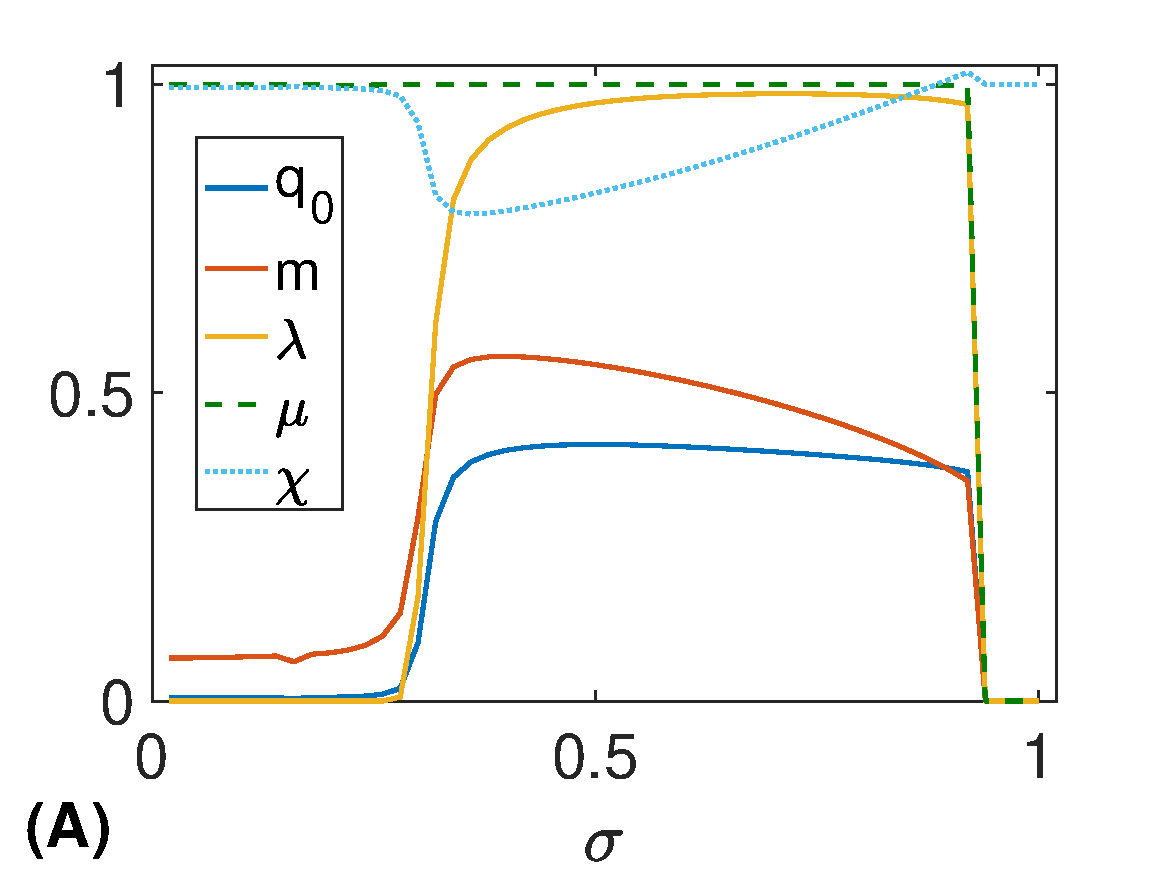
\includegraphics[scale=0.23]{fig1a.pdf}\,\,
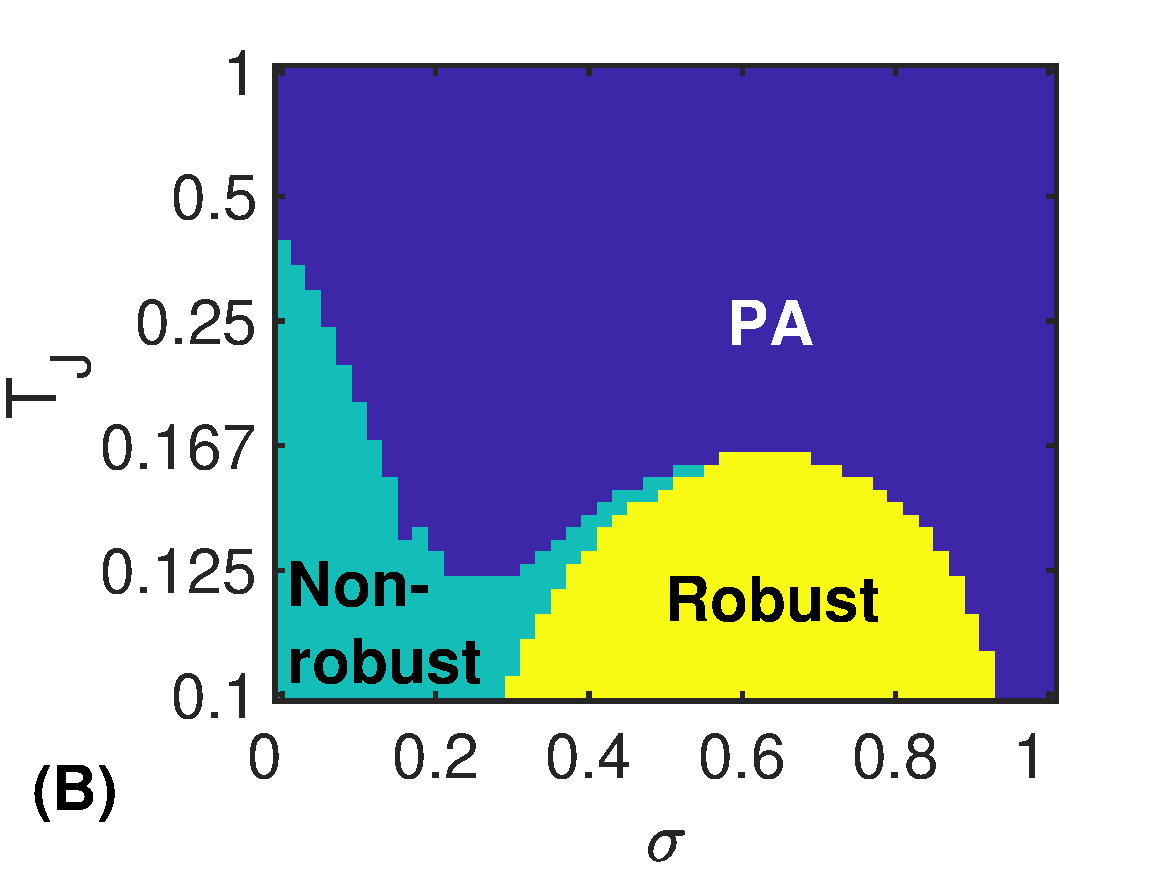
\includegraphics[scale=0.23]{fig2b-eps-converted-to.pdf}
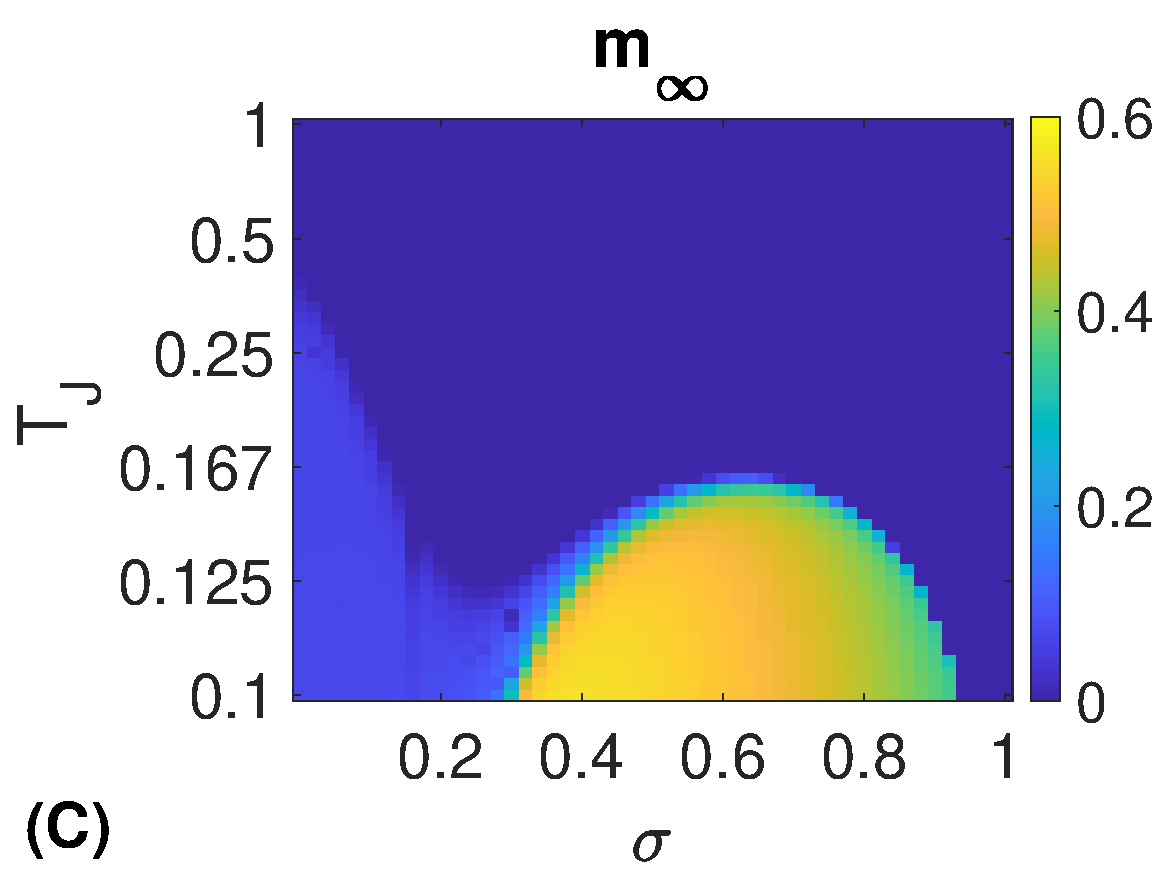
\includegraphics[scale=0.215]{fig2c.pdf}
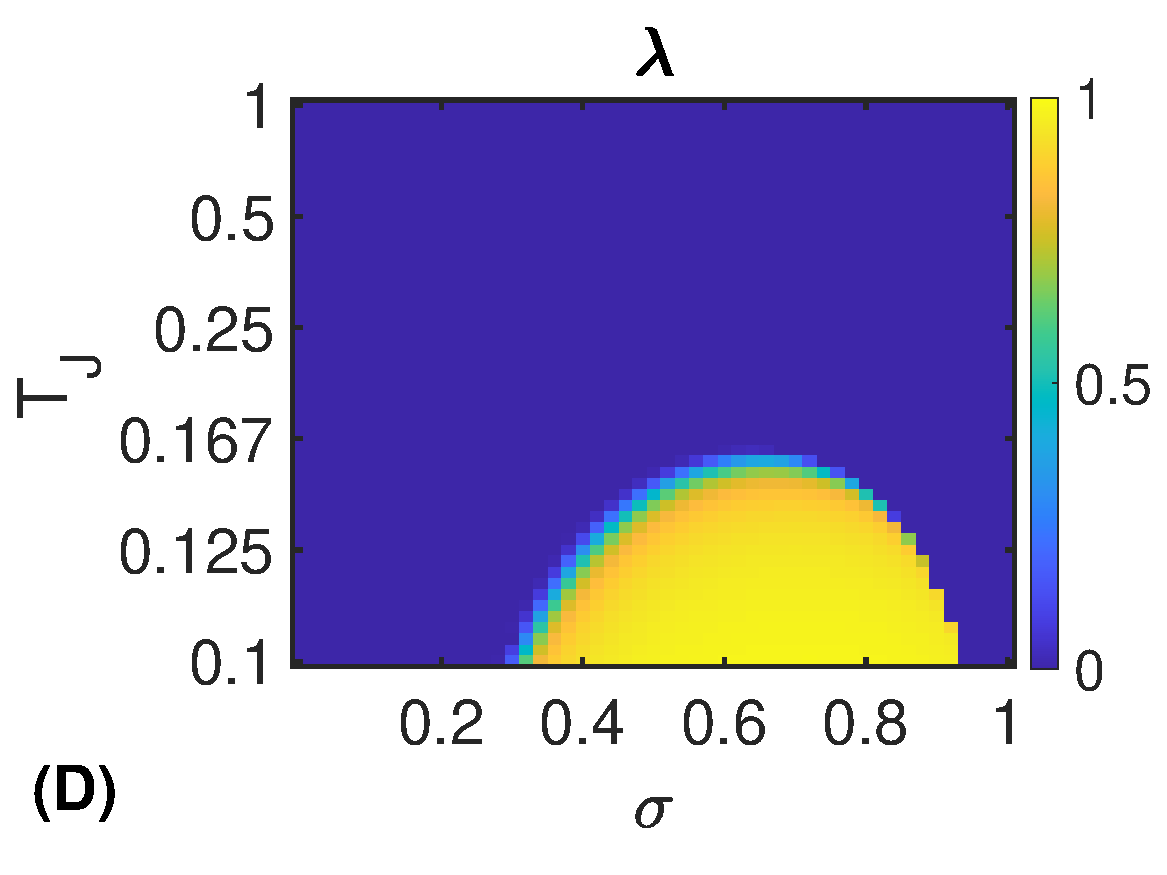
\includegraphics[scale=0.22]{fig2d-eps-converted-to.pdf}
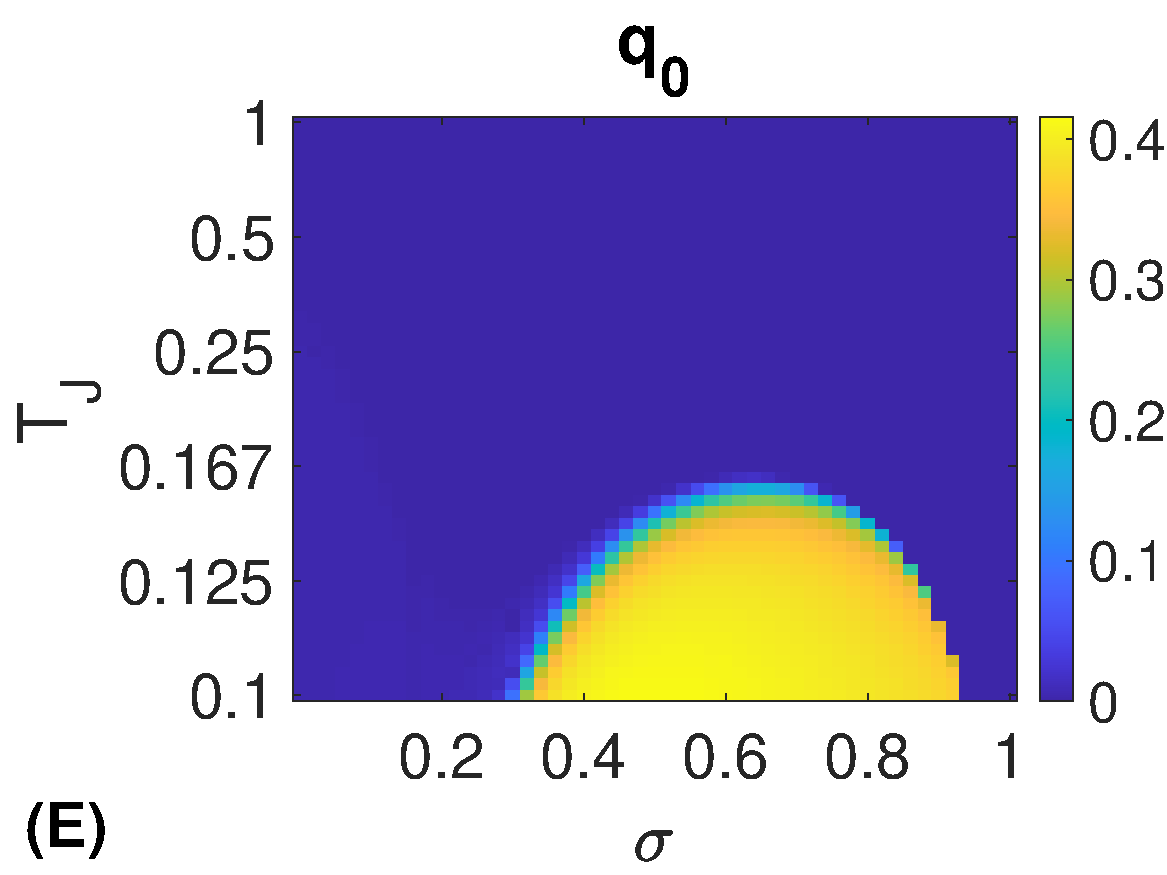
\includegraphics[scale=0.215]{fig2e.pdf}
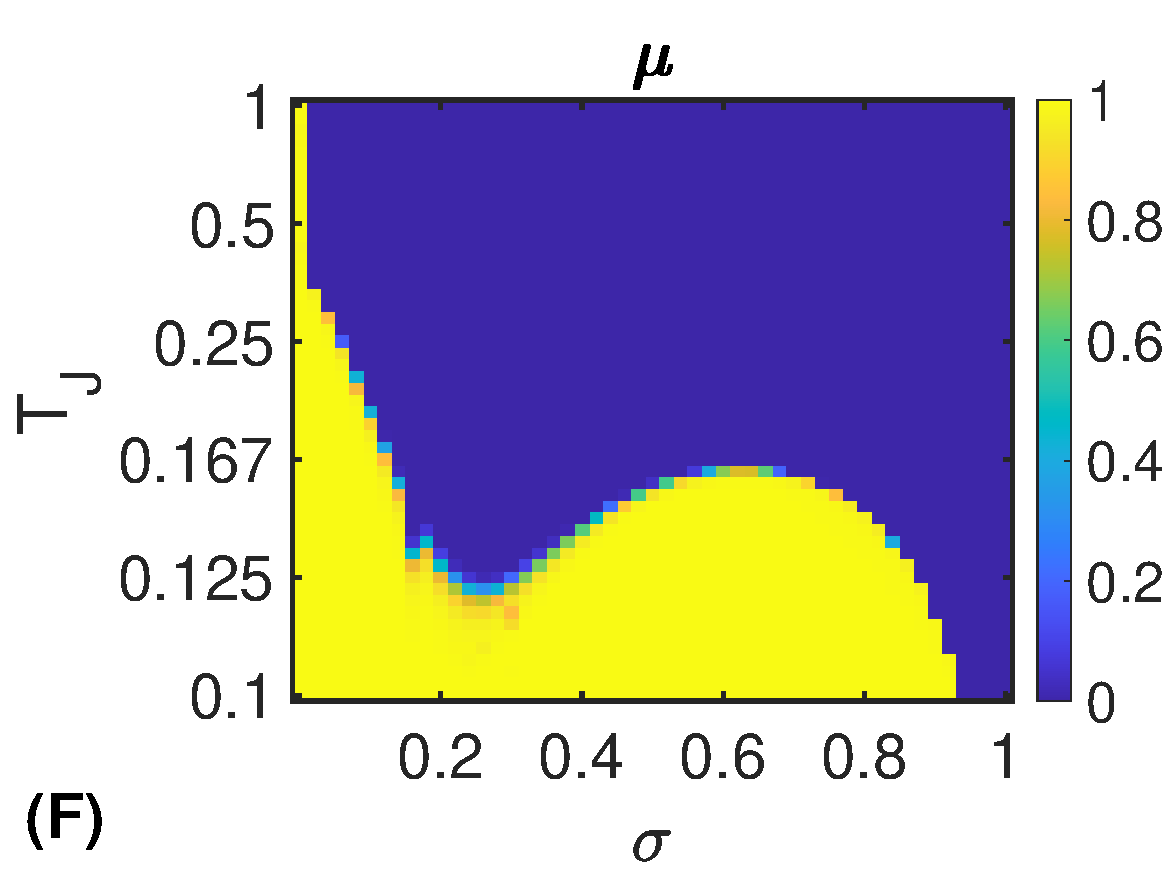
\includegraphics[scale=0.215]{fig2f-eps-converted-to.pdf}
\caption{\textbf{(A)} Order parameters  as function of $\sigma$ for $\beta=10$. In the non-robust phase $m >  0$ and $\mu =1$ but $\lambda = q_0= 0$, while in the robust phase    $m , q_0, \lambda, \mu >0$. In the para-attractor phase \textbf{(PA)}   $m = q_0 = \lambda = \mu=0$. \textbf{(B)} The  phase diagram in terms of $\sigma$ and $T_J =\beta^{-1}$. \textbf{(C)} Averaged activity of target genes $m$.  \textbf{(D)}  The average of target vs non-target coupling $\lambda$.  \textbf{(E)} The intrinsic variance in the  target gene's activity  $q_0$.  \textbf{(F)}  The  average of target vs target coupling $\mu$. Here $\alpha=0.5$.}  %In all panels $\alpha=0.5$.  } 
\label{fig:fig1}
\end{figure}

%In Fig. \ref{fig:fig1} we depict the order parameters as function of the noise strength $\sigma$ (left column) and $\alpha$ (right column) for a particular choice of $\beta=1$. In overall, the noise-dependence of the mean activity $m$  agrees with what was observed numerically in \cite{KanekoPloSOne2007} where, starting from some $\sigma_c(\alpha)$, $m$ increases upon increasing $\sigma$. 

 Let us recall  the meaning of the steady-state order parameters $m_{\infty}$, $q_0$, $\lambda$, $\mu$ and $\chi$. $m_{\infty}$ is the average of the \emph{random} fixed point $x_*$ as the latter depends on the realisation of both $z$ and $\tilde{z}$; $q_0$ is the variance of $x_*$ subtracted from $\sigma^2$, so that $q_0$ measures only the intrinsic fluctuation in $x_*$ that is not due to  the external noise $\sigma$. $\chi$ is the response of $x_*$ wrt perturbation induced by $z$; $\mu$ and $\lambda$ are the steady-state mean value of $J^{(tt)}$ and $J^{(to)}$. 
 
 The following result is presented for $\alpha=0.5$, similar behaviour is observed for other $\alpha \geq 0.08$ (see SM for the dependence of the order parameters on $\alpha$). At sufficiently high selection pressure, such as for $\beta = 10$,  we find that upon increasing the noise $\sigma$, two transitions happen between three different types  of solutions in Fig. 1  \textbf{(A)}.  The first solution is $q_0=\lambda =0$ and $m_\infty, \mu>0$, the second one corresponds to $q_0,m_\infty, \lambda, \mu >0$ and the last one -- to  $q_0=m_\infty= \lambda =\mu =0$. We call them non-robust, robust and para-attractor, respectively. Figure 1  \textbf{(B)} shows the full phase structure in terms of $T_J = 1/\beta$ and $\sigma$, supported by detailed behaviour of the order parameters in Fig. 1  \textbf{(C)}-  \textbf{(F)}.  %The meaning of each phase can be briefly discussed as follows:  
  At low noise,  a high fitness-selection effect ($\beta > 2$) leads to a small but non-zero  %system %is not ergodic,  resulting in the emergence of multiple fixed-points whose 
steady-state  mean expression level   ($m_\infty>0$)  due to a positive feedback (ensured by Hebbian-learning in Eq. \eqref{h_for_Jtt}) between the  positivity of $\mu$  and $m_\infty$.  %{\re(note that even the assumed  time-translational symmetry is broken in this case}.
 The structure of this non-robust region is  similar to that of a spin-glass phase at low-temperature % with replica-symmetry breaking, even though the dynamics  is not Hamiltonian. This seems to be
 because of the randomness in $J^{(to)}\sim \pm 1$ with the mean $\lambda =0$ acting on the target.   
 
 The robust region always exists within an intermediate range of noise strength $\sigma$, $\sigma \in \big[\sigma_c^{(1)}(T_J), \sigma_c^{(2)}(T_J)\big]$ below some $T_J$.   This phase can emerge if a sufficiently large noise  destabilises those stable fixed points observed at low noise. %The fraction of stable fixed point 
 Here phenotypes with high fitness  are achieved through the support of robust genotypes $J^{(tt)}$ and $J^{(to)}$, both, on average, remain close to 1, indicating the dominance of positive regulations \footnote{Note that since our calculations are restricted to the mean values of $J^{(tt)}$ and  $J^{(to)}$,  they can not be used to study how similar the evolved genotypes are in the robust phase}.  If  noise is increased further so that  the  diffusive term becomes much larger than the first term in Eq. \eqref{GRN_dynamics}, then  the loss of robustness occurs via a transition from the robust to para-attractor phase.
   In the para-attractor region, both phenotypic and genotypic values are zero, indicating the unique state is one that is neither robust nor functional. 
   
    The observed transitions are consistent with those  reported in the numerical evolution for finite systems \cite{KanekoPloSOne2007} where the robustnesses to noise and mutation that evolved at intermediate noise,  lost at lower noise, resulting in a less fitted frozen state. Likewise, we here find that the integrated response $\chi$ is reduced and  proportional to the response to mutation  \footnote{% the response to noise $G$ which is  the dynamical counterpart of the standard susceptibility and hence is a measure of how the averaged  expression level of $x(t)$ changes upon varying external term $\theta(t')$,  and obtained as %while the latter corresponds to its change upon changing $J_{ij}^{(tt)} \rightarrow J_{ij}^{(tt)} = J_{ij}^{(tt)}  + \delta J_{ij}^{(tt)} $. These  responses are given by
%\begin{equation}
%  G_{e}(t,t',\tau) :=  \frac{\partial \langle x(t,\tau) \rangle}{\partial \tilde{h}(t', \tau)} = -i \Big\langle  \hat{f}(t',\tau) x(t, \tau) \Big \rangle \label{thermal_response}
%\end{equation}
%with the  integrated responses  $
%   \chi_e = \int_0^t  dt' G_e(t,t',\tau) $
 In  case where the system has a non-zero  averaged activity $m >0$, as $t, \tau \rightarrow \infty$,
   $\chi \propto \chi_m := \sum_{\tau' = 0}^\tau G_m(t,\tau,\tau')$, where  $G_{m}(t, \tau, \tau') :=    \partial \langle x(t, \tau) \rangle\big/\partial \hat{\mu}(\tau')  $ is the response to mutation. Such proportionality between the two responses that implies a correlation between phenotypic changes due to genetic variation  and those in response to environmental perturbations, as suggested by \cite{KanekoPloSOne2007,Sato2003,Kaneko2006,Ciliberti, Sakata2020, Pham2022, Tang2021, Landry, Silva-Rocha, Uchida},  does not exist if  $m\simeq 0$.} in the robust phase, while it is larger at low noise regime.  Timeseries of $x$ in Eq. \eqref{closed1} in the robust and non-robust regions are given in Fig. 2, where the prediction of our fixed-point equations is found to be consistent with the timeseries  in  both regions. In particular, at low noise the deterministic system relaxes to a unique fixed point for any initial condition, while the small perturbation induced by $\sigma = 0.1$ results only in the proximity of random trajectories. The dynamics at intermediate noise $\sigma = 0.8$ exhibit intrinsic fluctuations that exist even when the external noise is removed. Nevertheless, despite of high variations in this case ($q_0\simeq 0.4$), the phenotypes  remain robust as shown by the dashed line indicating the mean expression level $m(t, \tau \rightarrow \infty)$.
\begin{figure}
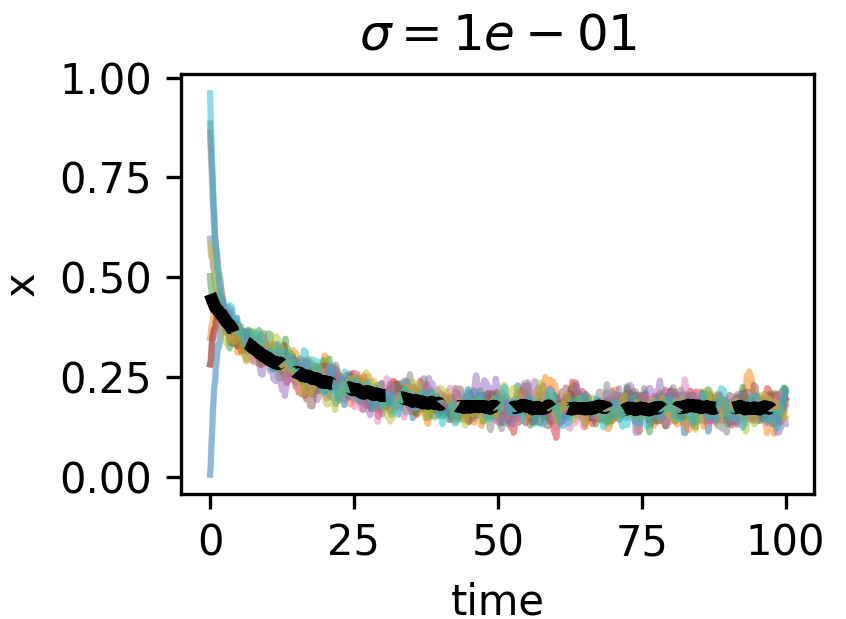
\includegraphics[scale=0.59]{Figure_2a.png}\,\,
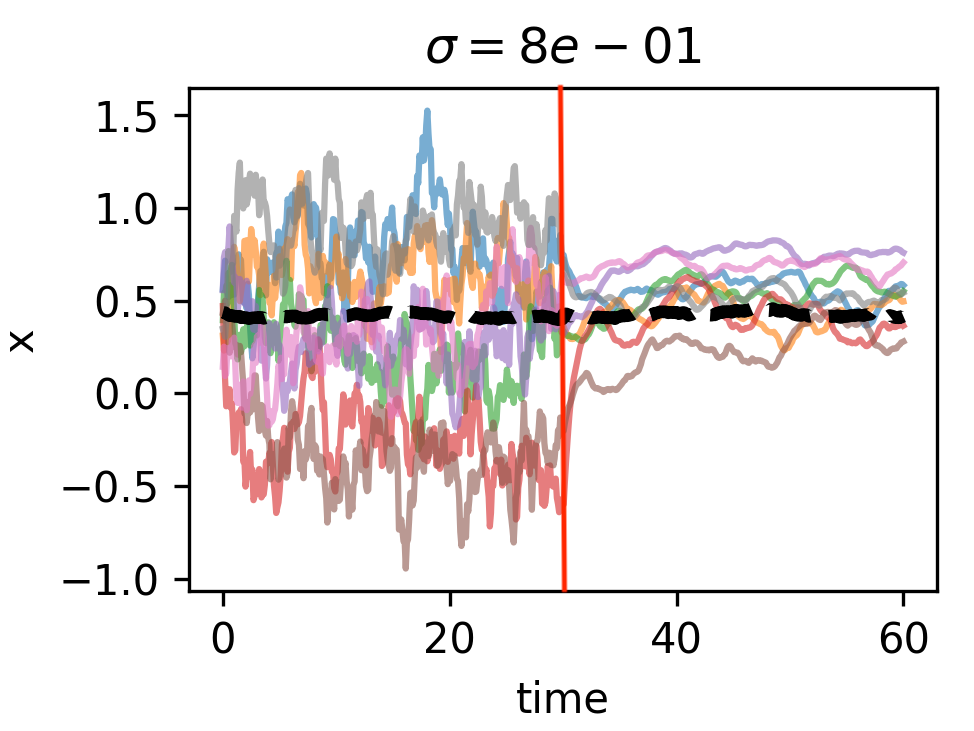
\includegraphics[scale=0.505]{Figure_2b}
\caption{Timeseries of the gene-expression level in the non-robust phase at low noise $\sigma = 0.1$ (left) and in the robust one at intermediate noise $\sigma = 0.8$ (right). In the plot with $\sigma = 0.8$   the vertical red line  marks the two stages of phenotypic evolution.  Here the timeseries for time $\in [0,30]$ are first generated at $\sigma = 0.8$, and then   continued after time $= 30$ by decreasing $\sigma$ to zero.  In all panels the thick dashed lines denote the mean expression level $m(t, \tau \rightarrow \infty)$ over $1000$ trajectories.} 
\label{fig:fig2}
\end{figure}

%The real critical behaviour, however, is observed once investigating the dependence of $m$ and $\chi$ on $\alpha$ in \ref{fig:fig1}, where a continuous phase transition occurs at a critical $\alpha_c(\sigma)$, though without any divergence of the integrated response $\chi$. This absence of diverging $\chi$ at criticality,  is, perhaps, due to the non-linearity imposed by the tanh function in comparison with a transition accompanied by the response' divergence observed in other models \cite{Galla2005, Galla2006}. Finally, to give a comprehensive picture of the model behavior in the full parameter range of interest, we plot all the order paramters in Fig. \ref{fig:fig2}. Using a classification based on the behaviour of $m$ and $\chi$, namely, $\alpha_c(\sigma)$ is identified as the point at which $m$ departs from zero and $\chi= \chi(\alpha)$ attain a maximum, we can distinguish two phases, robust and non-robust ones in Fig \ref{fig:fig3}.


%Correlation between variances of phenotypes due to noise and  genetic changes  has been discussed both in experiments and simulations %, and relationships to robustness have been discussed both theoretically .
%{\re Now we have confirmed the counter-intuitive result in \cite{KanekoPloSOne2007}, the loss of robustness at low noise regime.} 

   %, as it is proportional to the variance (i.e. the inverse of robustness). 
% Here mutations are defined as those change of the genotypes $J_{ij}$ that might happen spontaneously and independently from the dynamics specified previously. % Let $\delta x_i(\delta J_{jk})$ denote the change of the average local magnetisation of a target gene $i$ upon mutating a genotype  $J_{jk} \rightarrow J_{jk} + \delta J_{jk}$. The mutational response  of this target spin w.r.t such a change $M_{i,jk}$ then can be defined as $$M_{i,jk} = \lim_{\delta J_{jk} \rightarrow 0} \delta \Psi_i(\delta J_{jk})/ \delta J_{jk} = \big\langle s_is_js_k\big\rangle - \big\langle s_i\big\rangle  \big\langle s_js_k\big\rangle\,.$$In general, $J_{jk} \in\bold{J} = \bold{J}^{(tt)} \cup \bold{J}^{(oo)} \cup \bold{J}^{(to)}$. However, since fitness is determined solely by the configurations of target genes, we consider only  $J_{jk} \in \bold{J}^{(tt)}$ and  show that the average of this mutational response is equal to 
%We denote the response to perturbation by $G_e$ and that to mutation $G_m$. The former 
 % with multiple attractors. %due to the presence of a long-term memory as shown in SI.  
 %As argued in \cite{Sakata2020} such correlation can only be achieved in the replica symmetric region where the original high-dimensional dynamics of the phenotypes is reduced to a low-dimensional manifold due to evolution towards robustness. The variation of fitness due to noise and that due to mutation then happen to  occur along the same low-dimensional manifold, resulting in a correlation between them. {\re If RSB occurs, such restriction of  the  phenotypic dynamics no longer  exits, because in this case, changes of fitness upon varying the environmental conditions will vary arbitrarily from realisation to realisation of the $J_{ij}$'s dynamics.  As a result,  the system will have random, uncorrelated responses to noise and to mutations.}
\vskip0.2cm


% \section{Discussion}
 To sum up our ADMFT  demonstrated a robust-to-nonrobust transition with  decreasing noise, quantified by the set of order parameters.  The similarity between the nonrobust phase and spinglass, while noted,  needs future scrutiny. 
  %Some examples of systems where our approach might be applied include adaptive network models \cite{Gross2008}, cell differentiation  and reprogramming \cite{Waddington, Matsushita2022}, eco-evolutionary dynamics \cite{Post, Venkataram},  adaptive  integrate-and-fire model  of neuronal activity \cite{Brette2005} and Hopfield model with evolving patterns \cite{Schnaack}. 
From an evolutionary perspective, the term in Eq. \eqref{h_for_Jto} can be considered as what gives rise to epistasis \cite{Zhou2022}. %In general, within our framework we can study whether epistasis is a cause or a consequence of the genotype-phenotype mapping. 
 Moreover,  when subjected to  a time-dependent environment,  the fitted phenotypes  need to change over time, resulting in a more complicated %fitness is currently considered as a monotonic function of the mean activity of target genes, resulted in a single  optimal  phenotype but
relationship between  fitness and phenotypes  such as a  nonlinear dependence of $\Psi$ on $m$ due to a tradeoff between the cost and benefit \cite{Dekel2005}. 

 The  present ADMFT, beyond the genotype-phenotype evolution, can be applied to a wide class of adaptive systems, in which slow adaption of one type of degrees of freedom occurs in response to changes in the state of the other. Such reciprocal evolution is not captured by the standard DMFT that deals only with  fixed, i.e. ``quenched" coupling constants. Other extensions of DMFT  have been done recently  for neural dynamics with activity-dependent plasticity \cite{clark2023theory} and with  modification of synaptic
weights by external temporal patterns  \cite{Pereira-Obilinovic}. These approaches, however, are different from ours, where  a `learning' rule for the $\bold{J}$ variables  was derived from  a global fitness-maximization requirement. 
% induced by selection, 
The ADMFT further suggests the relevance of noise to shape robust memory by generating those evolved network structures that allow for the existence of an ensemble of intrinsically fluctuating  trajectories with constant mean. % {\re under Hebbian learning.  In fact,  according to  Eq. \eqref{h_for_Jto}, Hebbian learning for $J^{(to)}$ can only emerge when $J^{(to)} \simeq 1$  within intermediate noise.  Below the critical noise level,  the adaptation rule for $J_{ij}^{(to)}$ in Eq. \eqref{h_for_Jto} is non-Hebbian, resulting in  a loss of memory. 
%{\re Future work might establish a relation between the dynamics of learning and our  $\bold{J}$-dynamics based on fitness maximization.} %If this would be the case then gene-regulatory network can be considered as a kind of neural networks that is able to learn how to achieve robust pattern.
 
 %Mastrogiuseppe2017 % landscape  such as gene expression dynamics \cite{KanekoPloSOne2007} or neural networks with asymmetric couplings \cite{Schuecker2018, Mastrogiuseppe2017}. 
\bigskip

%https://www.overleaf.com/project/6353b6dc7c2bad368e9c3b72
\begin{acknowledgments}
We acknowledge support from Novo Nordisk Foundation (0065542) and would like to thank Albert Alonso, Julius B. Kirkegaard,  Kim Sneppen and Tarek Tohme, for stimulating discussions.
\end{acknowledgments}

\bibliography{Doublereplica}% Produces the bibliography via BibTeX.
 
\clearpage
 \appendix
 
 \onecolumngrid
 \section*{Supplemental material}
 \subsection*{A. Derivation of the effective dynamics in Eq. (4)} %\eqref{closed1}
Applying the Fourier transform to the probability distribution of paths  $\{x_k(t,\tau)\}$ generated by the gene-expression dynamics in Eq. (6) %\eqref{GRN_dynamics} 
$$\mathbb{P}_{{\rm traj}}\Big( \{x_k(t,\tau)\}\Big) := \mathbb{P}_{{\rm traj}}\Big[\big\{\mathbf{x}(0), \cdots, \mathbf{x}(t)\big\}_{\tau = 0}, \big\{\mathbf{x}(0), \cdots, \mathbf{x}(t)\big\}_{\tau = 1}, \cdots, \big\{\mathbf{x}(0), \cdots, \mathbf{x}(t)\big\}_{\tau = T} \Big]\,,$$
 with $T$ being the total number of generations (discrete time steps) of the $J$'s dynamics, we have the following identity
\begin{align} \nonumber
    1&= \int D\big[x\hat{x}\big]D\big[f\hat{f}\big] \exp\left\{i\cdot\sum_{\tau=0}^{T-1} \sum_{k=1}^{N} \int dt \Big[\hat{x}_k(t,\tau)\big(\partial_t +1 \big)x_k(t,\tau) + i\sigma^2\hat{x}_k^2(t,\tau)  - \gamma_k(t,\tau) \hat{x}_k(t,\tau)+ \hat{f}_k(t,\tau) \big(f_k(t,\tau) - z_k(t,\tau)\big) \Big] \right\} \\ 
     &= \int D\big[x\hat{x}\big]D\big[f\hat{f}\big] \exp\left\{i\cdot\sum_{\tau=0}^{T-1} \sum_{k=1}^N \int dt \Big[E_k(t, \tau) - \sum_{j=1}^N J_{kj}(\tau) \cdot\hat{f}_k(t,\tau) \cdot x_j(t, \tau) \big) \Big] \right\} \label{identity}
\end{align}
where  $J_{kk} = 0$ and
\begin{subequations}
\label{allequations4}
 \begin{eqnarray}
 z_k(t, \tau) &=& \tilde{h}_k(t) + \sum_{j(j\neq k)} J_{kj}(\tau) \cdot x_j(t,\tau) 
  \label{genedynamics1}
\\ \gamma_k(t,\tau) &=& {\rm tanh}\big(f_k(t,\tau) \big)
   \label{genedynamics2}
   \\ \int D[x\hat{x}]&=& \lim_{t_{\rm max}\rightarrow \infty} \int \prod_{k}^N \prod_{t}^{t_{\rm max}} \prod_{\tau}^{T-1} dx_k(t, \tau)  d\hat{x}_k(t, \tau) \label{genedynamics3} \\
E_k (t,\tau) &=& \hat{x}_k(t,\tau)\big(\partial_t +1 \big)x_k(t,\tau) +i\sigma^2 \hat{x}_k^2(t,\tau)- \gamma_k(t,\tau) \hat{x}_k(t,\tau) +\hat{f}_k(t,\tau) \big(f_k(t,\tau)  - \tilde{h}_k \big)\label{genedynamics4}
\end{eqnarray}
\end{subequations}
Note that, in the above expressions, $D\big[x\hat{x}\big]$ means  a measure over all the generations $\tau=0,\cdots, T$ of the $J$'s dynamics and over all   the possible paths of $x_k(t,\tau)$ and $\hat{x}_k(t,\tau)$ for all the genes at each of these generations, i.e. $D\big[x_k(t,\tau), \hat{x}_k(t,\tau)\big]$, $k=1,\cdots, N$. 
 We also used an integral representation of the probability $P(\xi)$ of the noise $\xi(t)$ with correlation $C_{\xi} =\langle \xi(t)\xi(t')\rangle = 2 \sigma^2\delta(t-t')$:
 $$P(\xi) \sim \exp\left[-\displaystyle\frac{1}{2} \int dt  dt'  \cdot\xi(t)\big[C_{\xi}(t,t')\big]^{-1} \xi(t') \right]$$
to write
\begin{align} \nonumber
1 &= \int Dx D\hat{x} D \xi P(\xi) \exp\left[ i \int dt\,  \hat{x}(t)\big[\partial_t x +x - \gamma(x(t), \tilde{h}(t)) - \xi(t) \big] \right] \\ \nonumber &= \int Dx D\hat{x} \exp\left[-\displaystyle\frac{1}{2} \int dt dt'\,  \hat{x}(t)C_{\xi}\hat{x}(t')+  i \int dt\,  \hat{x}(t)\big[\partial_t x +x - \gamma(x(t), \tilde{h}(t))  \big] \right]
\end{align}
%Generally, the \emph{time-dependent} local field $h_{kj}(\tau)$ can be decomposed into
%\begin{equation}
 %   h_{kj}(\tau)  = \underbrace{\theta_{kj}(\tau)}_{{\rm fitness}}\, + \underbrace{F_{kj}(\tau)}_{J-J\,{\rm interactions}} 
 %\label{local_field_for_coupling}
%\end{equation}
%We specify the fitness term as what is determined by the $x$'s dynamics 
%\begin{equation}
 %   \theta_{kj}(\tau) = \left[\frac{m_k(\tau) m_j(\tau)}{C_{kk}(\tau)}\right]^{1/2}\,,\qquad m_k(\tau) = \lim_{t\rightarrow \infty}\big\langle x_k(t,\tau) \big\rangle
  % \,,\qquad  C_{kk}(\tau) = \lim_{t,t'\rightarrow \infty}\big\langle x_k(t,\tau) x_k(t',\tau)\big\rangle\label{fitness_for_coupling}
%\end{equation}
%where $\langle \cdot \rangle$ denotes the average taken according to $\mathbb{P}_{{\rm traj}}\Big( \{x_k(t,\tau)\}\Big)$. 
 In equivalent to the dynamics of a single coupling in Eq. (2) %\eqref{coupling_dynamics},
 in case of synchronous update, the joint distribution $P(\bold{J})$ for the entire genotype satisfies a discrete-time master equation 
 \begin{align} \nonumber
P\big(\mathbf{J}(\tau+1)\big) &= \sum_{\mathbf{J}(\tau)} W_{\tau}\big[\mathbf{J}(\tau+1); \mathbf{J}(\tau)\big] P\big(\mathbf{J}(\tau)\big) 
\\ \nonumber W_{\tau}\big[\mathbf{J}(\tau+1); \mathbf{J}(\tau)\big] &= \prod_{k\neq j} W_{\tau}\big[J_{kj}(\tau+1); J_{kj}(\tau)\big] \\
   W_{\tau}\Big[J_{kj}(\tau+1); J_{kj}(\tau)\Big] & =  \frac{ e^{\displaystyle \beta J_{kj}(\tau+1)  h_{kj}(\mathbf{x}(\tau))}}{2 \, {\rm cosh}\big[\beta h_{kj}(\mathbf{x}(\tau)) \big]}\,.
\label{master_equation}
\end{align}
Without considering the $x$'s dynamics the moment generating functional of the trajectories  $\{\mathbf{J}(\tau)\}$, $\tau = 0,\cdots, T$,  according to Eq. \eqref{master_equation} reads
\begin{subequations}
\label{allequations5}
 \begin{eqnarray}
 Z_J[\mathbf{\Psi}] &=& \sum_{\{\mathbf{J}(0)\}} \cdots \sum_{\{\mathbf{J}(T)\}} \int D\big[h \hat{h}\big]
\exp\left\{\sum_{\tau=0}^{T-1} \sum_{k\neq j} A_{kj}(\tau)\right\}
  \label{generating_function1}
\\ 
   A_{kj}(\tau) &=& i\hat{h}_{kj}\big(h_{kj}-\theta_{kj}\big) +J_{kj}(\tau+1)\big(\Psi_{kj}(\tau+1) +\beta h_{kj}(\tau)\big) - \ln \big(2{\rm cosh}\, [\beta h_{kj}(\tau)]\big)\label{generating_function1b} \\
  \theta_{kj}^{(tt)}(\tau) & =&  \lim_{t\rightarrow \infty}\big\langle x_k(t,\tau) x_j(t,\tau)\big\rangle
   \\   \theta_{kj}^{(to)}(\tau) &=& \lim_{t\rightarrow \infty}\left\langle \big(1-x_k^2(t,\tau)\big)J_{kj}^{(to)}\Big(\sum_{\ell \in \mathcal{T}}J_{j \ell}^{(ot)}x_\ell(t,\tau)\right\rangle
\end{eqnarray}
\end{subequations}
Plugging Eq. \eqref{identity}  into \eqref{generating_function1} leads to 
\begin{equation}
    Z_J[\mathbf{\Psi}] = \int D\big[x\hat{x} f\hat{f} h \hat{h} \big] \sum_{\{\mathbf{J}(0)\}} \cdots \sum_{\{\mathbf{J}(T)\}} \exp\left\{\sum_{\tau=0}^{T-1} \left[i\cdot\sum_{k=1}^N \int dt E_k(t,\tau) + \sum_{k\neq j}\Big[  A_{kj}(\tau)-  i\, J_{kj}(\tau)\int dt \hat{f}_k x_j \Big]  \right]\right\}
\label{generating_function2}
\end{equation}
Denoting the $J$-independent and $J$-dependent part  of the exponential in $Z_J$ by $\mathcal{L}_0$ and $\mathcal{L}$, respectively. We have
\begin{subequations}
\label{allequations6}
 \begin{eqnarray}
 Z_J[\mathbf{\Psi}] &=& \int D\big[ x\hat{x} f\hat{f} h \hat{h} \big] e^{ \mathcal{L}_0} \cdot \left( \sum_{\{\mathbf{J}(0)\}} \cdots \sum_{\{\mathbf{J}(T)\}} e^{\mathcal{L}_J} \right)\\
     \mathcal{L}_0 &=&  \sum_{\tau=0}^{T-1} L(\tau)\\
     L(\tau) &=&  i\cdot\sum_k \int dt E_k(t,\tau) +\sum_{k\neq j} i\hat{h}_{kj}\big(h_{kj}- \theta_{kj}\big) - \sum_{k\neq j}  \ln \big(2{\rm cosh}\, [\beta h_{kj}(\tau)]\big) 
\\
     \mathcal{L}_J &=&  \sum_{\tau=0}^{T-1} \left[\sum_{k\neq j} J_{kj}\Big( \Psi_{kj} + \beta h_{kj} - i\int dt \hat{f}_k x_j \Big) \right]  
\end{eqnarray}
\end{subequations}
So far we have made no distinction between target and non-target genes. Now we  consider the following ansatz for any pair of target genes $k$ and $j$:
\begin{equation}
    J_{kj} = J^{(tt)}_{kj} + \Delta J_{kj}
\end{equation}
where $J^{(tt)}_{kj}$ is the direct interaction between $k$ and $j$ and $\Delta J_{kj}$ indicates the effective coupling between them that is induced by all the non-target genes $l$ via $J^{(to)}_{kl}$ and $J^{(to)}_{lj}$. In analogy to the standard quenched disorder case, where the  coupling $  J_{kj} $ is characterised by a distribution whose mean and  variance, both need to be scaled as $1/N_t$ for a sensible thermodynamic limit, we use
\begin{equation}
    J_{kj} = \frac{J^{(tt)}_{kj}}{N_t} + \Delta J_{kj}
\end{equation}
where $J^{(tt)}_{kj} \in \{ -1,1 \}$ and $
   \Delta J_{kj} = N_t^{-1}\sum_{l\centernot \in \mathcal{T}} J^{(to)}_{kl} J^{(to)}_{lj}$, with $J^{(to)}_{kj} \in \left\{ -1, 1\right\}$. The sum over $\{\mathbf{J}(\tau)\}$ in Eq. \eqref{generating_function2} can now be performed 
 to obtain
 %$$+ \sum_{k\in \mathcal{T}, l\centernot \in \mathcal{T}} \,J^{(to)}_{kl} \big(\Psi_{kl} + \beta H_{kl}\big)  - i\int  \frac{dt}{N_o} \sum_{k\neq j\in \mathcal{T}}\Big(\sum_{l\centernot \in \mathcal{T}} J^{(to)}_{kl} J^{(to)}_{lj}\Big)\hat{f}_k x_j  $$
 \begin{equation}
   S := \ln\left\{\sum_{\big\{J^{(tt)}_{kj}\big\}} \sum_{\big\{J^{(to)}_{kl}\big\}}  \exp ( \mathcal{L}_J) \right\}  =\sum_{\tau=0}^{T-1} S(\tau)\,,\qquad  S(\tau) = B(\tau) +  D(\tau)  
\label{generating_function4a}
\end{equation}
where, by defining the order parameters
\begin{subequations}
\label{allequations7}
 \begin{eqnarray}
 w_{kj}(\tau) &= &\frac{1}{N_t}\int dt  \hat{f}_k(t,\tau) x_j(t,\tau)
  \label{auxiliary1}
\\  m(t,\tau) & =&  \frac{1}{N_t}\sum_j x_j (t,\tau) 
  \label{auxiliary2}
  \\  g(t,\tau) &=& \frac{1}{N_t}\sum_k \hat{f}_k (t,\tau) 
  \label{auxiliary3} 
  \\ q(t,t',\tau) &= &  \frac{1}{N_t}\sum_{k} x_k(t,\tau) x_k(t',\tau)
  \label{auxiliary4}
\\ Q(t,t',\tau) &= & \frac{1}{N_t}\sum_{k} \hat{f}_k(t,\tau) \hat{f}_k(t',\tau) 
  \label{auxiliary5}
  \\ K(t,t',\tau) &= &  \frac{1}{N_t}\sum_{k} x_k(t,\tau) \hat{f}_k(t',\tau)
  \label{auxiliary6}
\end{eqnarray}
\end{subequations}
and using the identity $
     \sum_{k\neq j} w_{kj}(\tau) = N_t\int dt \cdot m(t,\tau) \cdot g(t,\tau)$,
%\begin{equation}
 %1 = \int D[w \hat{w}] D\big[m \hat{m}\big] D\big[g\hat{g}\big] \prod_{\tau=0}^{T-1}\exp\left\{iN S_0 + i\hat{w}(\tau)\Big(\sum_{k\neq j} w_{kj}(\tau)\Big)  - i\cdot\sum_k \int dt \Big[\hat{m}(t,\tau) x_k(t,\tau) +\hat{g}(t,\tau)\hat{f}_k(t,\tau)\Big]\right\}  
%\end{equation}
we can compute
\begin{align}
\nonumber   B(\tau) &= \ln\left\{ \int D[\hat{\mu}w m g] \exp\left( i\hat{\mu}(\tau) \left[N_t\int dt\cdot m(t,\tau)g(t,\tau) + \sum_{k\neq j} w_{kj}(\tau) - \sum_k \int dt \Big[g(t,\tau)x_k(t,\tau) + m(t,\tau)\hat{f}_k(t,\tau)\Big]  \right]      \right) \right\} \\
  &+ \sum_{k\neq j \in \mathcal{T}} \ln 2{\rm cosh}\,\left(\frac{\Psi_{kj}(\tau+1) +\beta h_{kj}(\tau)}{N_t} - i w_{kj}(\tau) \right) 
\end{align} 
\begin{align} \nonumber
    D(\tau) &= \ln\left\{ \sum_{\displaystyle \Big\{J^{(to)}_{kl} = \pm 1\Big\}}    \exp\left\{\displaystyle \,\sum_{k\in \mathcal{T},    l\centernot \in \mathcal{T} } J^{(to)}_{kl} \big(\Psi_{kl}+ \beta h_{kl}\big)  -i \sum_{k\neq j \in \mathcal{T}}\left[\int dt \Big(\frac{1}{N_t}\sum_{ l\centernot \in \mathcal{T}} J_{kl}^{(to)}J_{lj}^{(to)}  \Big) \hat{f}_k x_j\right] \right\}\right\} 
   \\ \nonumber
   &= \ln\left\{ \sum_{\displaystyle \Big\{J^{(to)}_{kl} = \pm 1\Big\}}    \exp\left\{\displaystyle \,\sum_{k\in \mathcal{T},    l\centernot \in \mathcal{T} } J^{(to)}_{kl} \big(\Psi_{kl}+ \beta h_{kl}\big)  -i \sum_{ l\centernot \in \mathcal{T}} \int dt \left[ \Big(\sum_{k \in \mathcal{T}} \frac{J_{kl}^{(to)}}{\sqrt{N_t}} \hat{f}_k \Big) \ \cdot \Big(\sum_{j \in \mathcal{T}} \frac{J_{lj}^{(to)} }{\sqrt{N_t}}x_j \Big)  \right] \right\}\right\} \\ \nonumber
   &= \ln\left\{\sum_{\displaystyle \Big\{J^{(to)}_{kl} \Big\}}   \prod_{l\centernot \in \mathcal{T}} \left[\int Dy_l Dz_l\cdot \exp\left\{\displaystyle -i \int dt y_lz_l + \,\sum_{k\in \mathcal{T}} J_{kl}\frac{\Psi_{kl}+ \beta h_{kl}}{\sqrt{N_t}}\right\} \cdot \int dt \, \delta\Big(z_l- \sum_{k\in \mathcal{T}} \frac{J_{kl}}{\sqrt{N_t}} \hat{f}_k\Big) \cdot \delta\Big(y_l- \sum_{j\in \mathcal{T}} \frac{J_{jl}}{\sqrt{N_t}}x_j\, \Big)     \right]\right\} 
  \\\nonumber &= \ln\left\{\int D\big[y\hat{y}\big] D\big[z\hat{z}\big]\cdot e^{\displaystyle i\int dt\sum_{l\centernot \in \mathcal{T}}[z_l\hat{z}_l + y_l\hat{y}_l-z_ly_l ]}    \sum_{\big\{J_{kl}\big\}} \exp\left\{\sum_{k\in \mathcal{T}, l\centernot \in \mathcal{T}} \frac{J_{kl} }{\sqrt{N_t}} \left[\Psi_{kl}+ \beta h_{kl}-i \int dt \, \big(\hat{z}_l \hat{f}_k + \hat{y}_lx_k\big)\right]\right\} \right\} \\ \nonumber &= \ln\left\{\int D\big[y\hat{y}\big] D\big[z\hat{z}\big]\cdot \exp\left\{\displaystyle i\int dt\sum_{l\centernot \in \mathcal{T}}[z_l\hat{z}_l + y_l\hat{y}_l-z_ly_l ]     +\sum_{k,l} \ln\left[ {\rm cos}\left( i \cdot \frac{\Psi_{kl}+ \beta h_{kl}}{\sqrt{N_t}}   +  \int dt \frac{\hat{z}_l\hat{f}_k +\hat{y}_lx_k}{\sqrt{N_t}}  \right)     \right]\right\}\right\} \\  &= \ln\left\{\int D\big[y\hat{y}\big] D\big[z\hat{z}\big] D\big[q\hat{q}\big] D\big[Q\hat{Q}\big]
    D\big[K\hat{K}\big]\cdot \exp\left(N_t\Big[ \displaystyle  i\psi +  \Phi +  \Omega \Big]  + \int dt\sum_{l\centernot \in \mathcal{T}}[z_l\hat{z}_l + y_l\hat{y}_l-z_ly_l]\right)\right\} 
\end{align}
where
\begin{subequations}
\label{allequations8}
 \begin{eqnarray*}
\psi &=&   \int dt dt'\left\{ q\cdot \left[\hat{q} + \frac{i}{2N_t} \,  \sum_{l\centernot \in \mathcal{T}}\hat{y}_l(t)\hat{y}_l(t') \right]+ Q\cdot \left[\hat{Q}  +  \frac{i }{2N_t} \,\sum_{l\centernot \in \mathcal{T}} \hat{z}_l(t)\hat{z}_l(t')\right] +  K\cdot  \left[ \hat{K} + \frac{i}{N_t} \sum_{l\centernot \in \mathcal{T}}\hat{y}_l(t)\hat{z}_l(t') \right] \right\}  \\
\Phi &=& -\frac{i}{N_t}  \sum_k \int dt dt'\left[\hat{q}\cdot    x_k(t)x_k(t') +\hat{Q}\cdot  \hat{f}_k(t)\hat{f}_k(t')\ + \hat{K}\cdot  \hat{f}_k(t')x_k(t) \right] \\ 
\Omega  &=& \frac{1}{N_t^2} \sum_{k \in \mathcal{T},l \centernot \in \mathcal{T}} \left[  \frac{\big(\Psi_{kl} + \beta h_{kl}\big)^2} {2} - i\big(\Psi_{kl} + \beta h_{kl}\big) \int dt \cdot \big(\hat{z}_l\hat{f}_k +\hat{y}_lx_k\big) \right]
\end{eqnarray*}
\end{subequations}
Substituting $\hat{y} = z$ and $\hat{z} = y$, those that are obtained by varying the action wrt $y$ and $z$, respectively, we get
\begin{subequations}
\label{allequations9}
 \begin{eqnarray*}
\psi &=&   \int dt dt'\left\{ q\cdot \left[\hat{q} + \frac{i }{2N_t} \,\sum_{l\centernot \in \mathcal{T}} z_l(t)z_l(t') \right]+ Q\cdot \left[\hat{Q}  +  \frac{i}{2N_t} \,\sum_{l\centernot \in \mathcal{T}} y_l(t)y_l(t')\right] +  K\cdot  \left[ \hat{K} + \frac{i}{N_t} \,\sum_{l\centernot \in \mathcal{T}}z_l(t)y_l(t') \right] \right\}  \\
\Omega &=&  \frac{1}{N_t^2} \sum_{k \in \mathcal{T},l \centernot \in \mathcal{T}} \left[  \frac{\big(\Psi_{kl} + \beta h_{kl}\big)^2} {2} - i\, \big(\Psi_{kl} + \beta h_{kl}\big) \int dt \cdot \big(z_l x_k + y_l\hat{f}_k\big) \right]
\end{eqnarray*}
\end{subequations}
Saddle-point conditions for $\big (\psi + \Phi \big)$ wrt $q, Q$ and $K$; $\hat{q}, \hat{Q}$ and $\hat{K}$ lead to
\begin{equation}
        \left \{ \begin{array}{l} \displaystyle \frac{\partial \psi}{\partial q} = 0\,,\quad \rightarrow \hat{q}_* = -\frac{i \alpha}{2}\cdot\langle z(t)z(t')\rangle_* \\ \\ \displaystyle \frac{\partial \psi}{\partial Q} = 0\,,\quad \rightarrow  \hat{Q}_* = -\frac{i\alpha }{2}\cdot \langle y(t)y(t')\rangle_*\\ \\ \displaystyle  \frac{\partial \psi}{\partial K} = 0\,,\quad  \rightarrow \hat{K}_* = -i\alpha\cdot \langle z(t)y(t') \rangle_*
     \end{array} \right.\, \,,\qquad 
\left \{ \begin{array}{l}  \displaystyle \frac{\partial (\psi + \Phi \big)}{\partial \hat{q}} = 0 \,,\quad \rightarrow  q = \big\langle  x(t) x(t') \big\rangle_* \\ \\\displaystyle \frac{\partial (\psi + \Phi \big)}{\partial \hat{Q}} = 0  \,,\quad  \rightarrow Q = \langle \hat{f}(t) \hat{f}(t')\rangle_*  \\ \\ \displaystyle \frac{\partial (\psi + \Phi \big)}{\partial \hat{K}} = 0  \,,\quad  \rightarrow K = \langle x(t)  \hat{f}(t') \rangle_*  \end{array} \right.\,,
\end{equation}
where $\alpha = N_o/N_t$ and we have   introduced a  measure for the effective dynamics of a single gene $x$ that evolves under all realizations of $\Big(x, \hat{x}, f, \hat{f}, h, \hat{h},   w, \hat{w} \Big)$ as
\begin{equation}
\Big\langle O\big(x, \hat{x}, f, \hat{f},h, \hat{h},w,\hat{w}\big) \Big\rangle = \frac{\displaystyle \int  Dy Dz D\big[x \hat{x} f \hat{f} h \hat{h} w \hat{w} \big]\cdot O \cdot e^{L}}{\displaystyle  \int   Dy Dz D\big[x \hat{x} f \hat{f}  h \hat{h} w \hat{w} \big] e^{L} } \,,\qquad L = \sum_{\tau =0}^{T-1} L(\tau) + S(\tau) 
\end{equation}
where
\begin{subequations}
\label{allequations10}
 \begin{eqnarray}
 L(\tau) + S(\tau) &=& \sum_{k\neq j \in \mathcal{T}} W_{kj}  + \sum_{k \in \mathcal{T}, l \centernot \in \mathcal{T}} \tilde{W}_{kl} +   i\sum_k  \left(\int dt E_k(t,\tau) - M_k^{(\rm sd)} (\tau) \right) \\
M_k^{(\rm sd)} (\tau) &=& \hat{\mu}(\tau)  \int dt \big[g_* x_k + m_*\hat{f}_k\big] + \int dt dt'\left[\hat{q}_*\cdot    x_k(t)x_k(t') +\hat{Q}_*\cdot  \hat{f}_k(t)\hat{f}_k(t')\ + \hat{K}_*\cdot  \hat{f}_k(t')x_k(t) \right] \\W_{kj} &=& i\hat{h}_{kj}^{(tt)}\big(h_{kj}^{(tt)}-\theta_{kj}\big) +  \ln\left[\frac{2{\rm cosh}\,\left(\displaystyle \frac{\Psi_{kj}(\tau+1) +\beta h_{kj}^{(tt)}(\tau)}{N_t} - i w_{kj}(\tau)\right)}{ 2{\rm cosh}\, \big[\beta h_{kj}^{(tt)}(\tau)/N_t\big]}\right] \\\tilde{W}_{kl} & =& \frac{\big(\Psi_{kl} + \beta h_{kl}^{(to)}\big)^2} {2N_t} - i\frac{\Psi_{kl} + \beta h_{kl}^{(to)}}{N_t} \int dt  \big[y\hat{f}_k + z x_k\big]  + i\hat{h}_{kl}^{(to)} \big(h_{kl}^{(to)} -\tilde{\theta}_{kl}\big) - \ln\Big[2{\rm cosh}\, \Big(\frac{\beta h_{kl}^{(to)}}{\sqrt{N_t}} \Big)\Big] 
\end{eqnarray}
\end{subequations}

%Considering the limit $\Psi \rightarrow 0$, and using $H_{kl} = \lambda(m)$, one can consider
%$$R_l=  - \frac{i}{\sqrt{N_0}}\,  \sum_k  \int dt \cdot \big[y\hat{f}_k + z x_k\big] = -i\alpha\,\sum_{j,k} J_{jl} \int dt\frac{\big[ x_j \hat{f}_k +      x_k \hat{f}_j\big]}{N} = -i\alpha\,\sum_{j} J_{jl} \int dt \big[g x_j  +      m \hat{f}_j\big] $$
%Hence in this limit
%$$\tilde{W}_{kl}\big|_{\Psi \rightarrow 0} = \frac{\big( \beta H_{kl}\big)^2} {2} -i\alpha\, \big( \beta H_{kl}\big) J_{kl} \int dt \big[g x_k  +      m \hat{f}_k\big] + i\hat{H}_{kl} \big(H_{kl} -\tilde{\theta}_{kl}\big) - \ln\Big(2{\rm cosh}\, \big(\beta H_{kl}\big)\Big)   $$
Saddle-point conditions for $\tilde{W}= \sum_{k,l} \tilde{W}_{kl}$ wrt $h_{kl}^{(to)}$ and $\hat{h}_{kl}^{(to)}$ in the limit $\Psi_{kl} \rightarrow 0$  lead to
%\begin{equation}
  %      \left \{ \begin{array}{l} \displaystyle \frac{\partial \tilde{W}}{\partial h_{kl}^{(to)}} = 0\,,\quad \rightarrow  \frac{\beta^2}{N_t} h_{kl}^{(to)}  + i\, \hat{h}_{kl}^{(to)} - \frac{ \beta}{\sqrt{N_t}}{\rm tanh}\,\Big(\frac{ \beta}{\sqrt{N_t}}  h_{kl}^{(to)}\Big) -\frac{i \beta}{N_t} \int dt \cdot \big[y \hat{f}_k + z x_k\big] =0 \\ \\ \displaystyle \frac{\partial \tilde{W}}{\partial \hat{h}_{kl}^{(to)}} = 0\,,\quad \rightarrow  h_{kl}^{(to)} = \tilde{\theta}_{kl}
 %    \end{array} \right.\, 
%\end{equation}
%From these equations  %first among these 
%we get
%$$\frac{\beta}{\sqrt{N_t}} h_{kl}^{(to)}  - \, {\rm tanh}\,\Big(\frac{ \beta}{\sqrt{N_t}}h_{kl}^{(to)}\Big) = \frac{i}{\sqrt{N_t}} \int dt \cdot \big[y \hat{f}_k + z x_k\big]$$
%On the other hand,$$\Big \langle J^{(to)}_{kl} \Big\rangle = \lim_{\Psi\rightarrow 0} \frac{\partial Z}{\partial \Psi_{kl}} =  \frac{\beta}{N_t} h_{kl}^{(to)} - \frac{i}{N_t} \int dt \cdot \big[y \hat{f}_k + z x_k\big] $$
%Therefore,
\begin{equation}
  \hat{\lambda}(\tau+1)  := \sqrt{N_t}  \Big\langle J^{(to)}_{kl}(\tau+1) \Big\rangle = \sqrt{N_t} \left(\lim_{\Psi\rightarrow 0}  \frac{\partial Z}{\partial \Psi_{kl}}\right)  ={\rm tanh}\,\left(\frac{ \beta}{\sqrt{N_t}} h_{kl}^{(to)}(\tau)\right)  
\end{equation}
Similar saddle-point calculations for $W= \sum_{k,j} W_{kj}$  yield $ h_{kj}^{(tt)}(\tau) = \theta_{kj}(\tau)$ and 
\begin{equation}
   \Big \langle   J^{(tt)}_{kj}(\tau+1) \Big\rangle  :=\lim_{\Psi\rightarrow 0} \frac{\partial Z}{\partial \Psi_{kj}} = \frac{1}{N_t}{\rm tanh} \left(\frac{ \beta}{N_t} h_{kj}^{(tt)}(\tau)\right)\,,\qquad  \rightarrow \hat{\mu}(\tau+1) =  {\rm tanh} \left(\frac{ \beta}{N_t} h_{kj}^{(tt)}(\tau)\right)
\end{equation}
The final step consists of evaluating these $\hat{q}_*,   \hat{Q}_*,  \hat{K}_* $ as follows
\begin{align}\nonumber
    \hat{q}_* &= -\frac{i \alpha }{2 }\left\langle\left(\sum_{\ell'\in \mathcal{T}} J_{\ell'}^{(to)}\hat{f}_{\ell'}(t) \right)\left(\sum_{\ell \in \mathcal{T}}J_{\ell}^{(to)}\hat{f}_{\ell}(t')  \right) \right\rangle_* = -\frac{i\alpha}{ 2}\left(\sum_{\ell' \neq \ell} J_{\ell'}^{(to)}J_{\ell}^{(to)}\left\langle \hat{f}_{\ell'}(t)  \hat{f}_{\ell}(t') \right \rangle_*+ \sum_{\ell \in\mathcal{T}} \big[J_{\ell}^{(to)}\big]^2  \left\langle\hat{f}_{\ell}(t)  \hat{f}_{\ell}(t')\right \rangle_* \right)= 0 \\
\nonumber
    \hat{Q}_* &= -\frac{i \alpha}{2 }\left\langle\left(\sum_{\ell'} J_{\ell'}^{(to)}x_{\ell'}(t)  \right)\left(\sum_\ell J_{\ell}^{(to)}x_{\ell}(t')  \right) \right\rangle_* = -\frac{i\alpha}{ 2}\left(\sum_{\ell' \neq \ell} J_{\ell'}^{(to)}J_{\ell}^{(to)}\big\langle x_{\ell'}(t)  x_{\ell}(t') \big\rangle_*+ \sum_{\ell} \big[J_{\ell}^{(to)}\big]^2  \big\langle x_{\ell}(t)  x_{\ell}(t')\big \rangle_* \right) \\ \nonumber&=- \frac{i\alpha  \lambda^2}{2 } C(t,t')
\\ \nonumber
    \hat{K}_* &= - i \alpha\left\langle\left(\sum_{\ell'} J_{\ell'}^{(to)}\hat{f}_{\ell'}(t)  \right)\left(\sum_\ell J_{\ell}^{(to)}x_{\ell}(t')  \right) \right\rangle_* = -i\alpha\left(\sum_{\ell' \neq \ell} J_{\ell'}^{(to)} J_{\ell}^{(to)}\left\langle \hat{f}_{\ell'}(t)  x_{\ell}(t') \right \rangle_*+ \sum_{\ell} \big[J_{\ell}^{(to)}\big]^2 \underbrace{ \left\langle \hat{f}_{\ell}(t)  x_{\ell}(t')\right \rangle_*}_{\displaystyle K(t',t)} \right) \\ &= - i\alpha \lambda^2  \,\Big(i \underbrace{\frac{\partial \big\langle x(t')\big\rangle_*}{\partial \tilde{h}(t)}}_{\displaystyle G(t',t)}\Big)
\end{align}
The effective single-gene dynamics is generated by the following path probability, introducing the notation, $\hat{\mu} = \hat{w}$,
\begin{align} \nonumber  P(x(t)) & = \int D\big[x\hat{x} f \hat{f}\big] \prod_{\tau =0}^{T-1}\left[ \exp\Big\{ i\cdot \int dt \Big[ \hat{x} \big(\partial_t + 1 \big)x +i\sigma^2 \hat{x}^2 - \hat{x}\gamma(f)  + \hat{f}\big(f-  m_*\hat{\mu}(\tau)  - \tilde{h} \big) \Big] \right. \\ &- \left.  \alpha \hat{\lambda}^2(\tau)   \int dt dt' \Big[ \frac{C(t,t')}{2} \hat{f}(t)\hat{f}(t') + iG(t',t)x(t)\hat{f}(t')\Big]\Big\}\right]
\end{align}
 This equation results  in the equivalent SDE form of Eq. (4). %\eqref{closed1}.
%\section{B. Additional results}
 In addition to the results in the main text, here we present the model phase diagrams in terms of $\alpha$ and $\sigma$ in Fig. 3.
 \begin{figure}[b]
 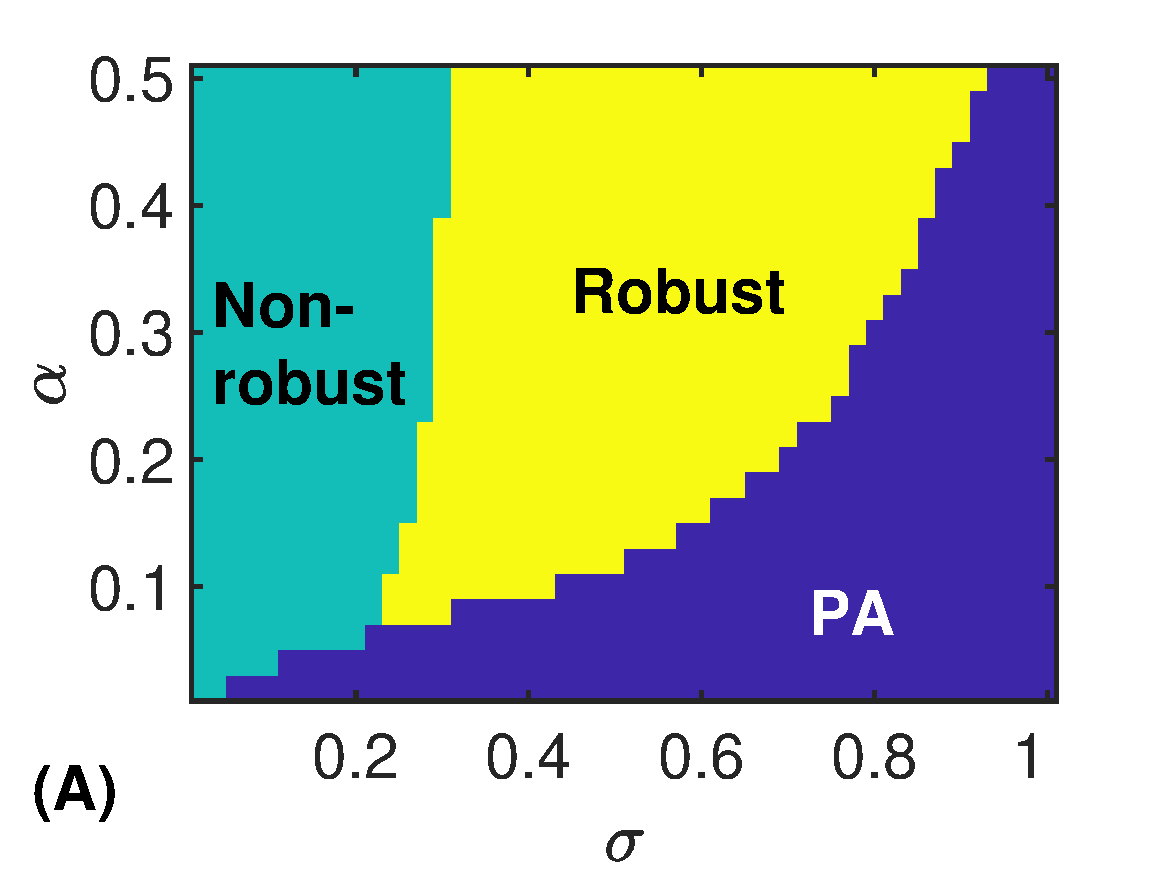
\includegraphics[scale=0.22]{fig2a-eps-converted-to.pdf}
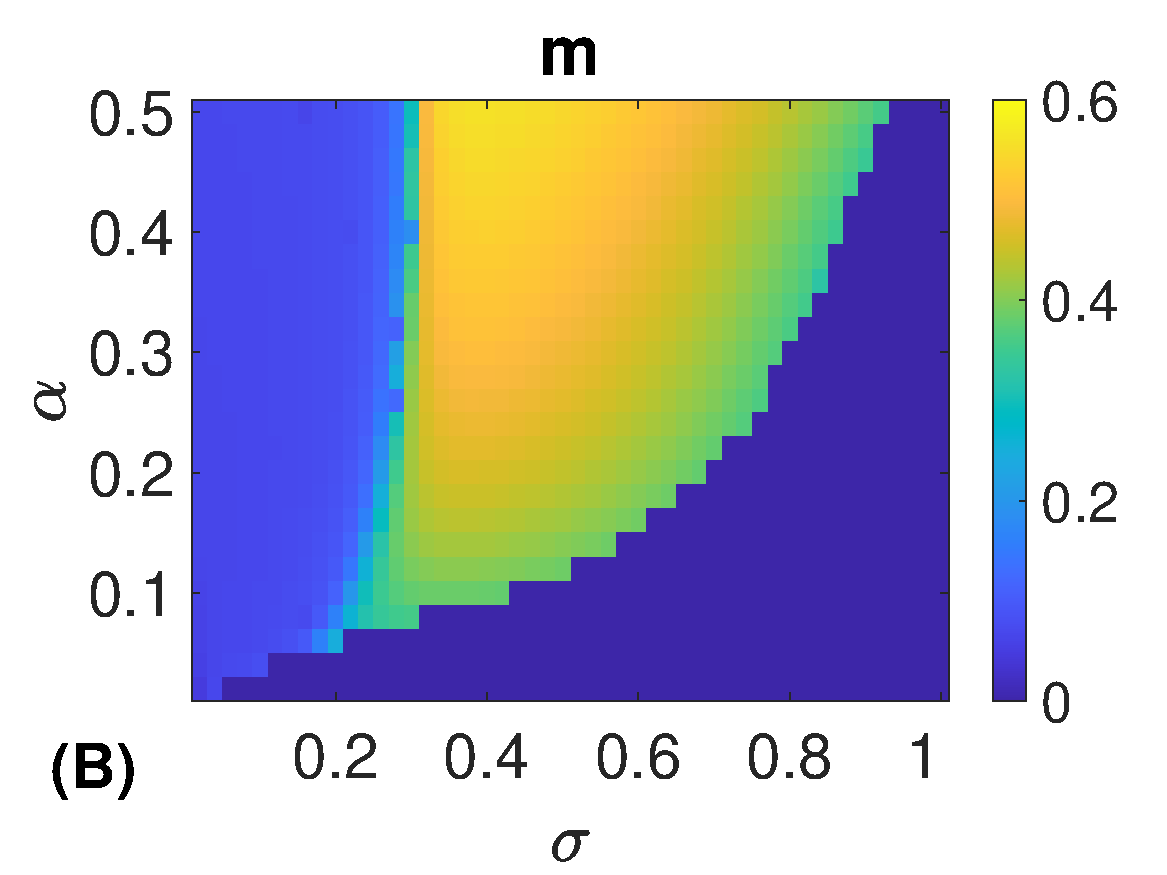
\includegraphics[scale=0.22]{fig1b-eps-converted-to.pdf}
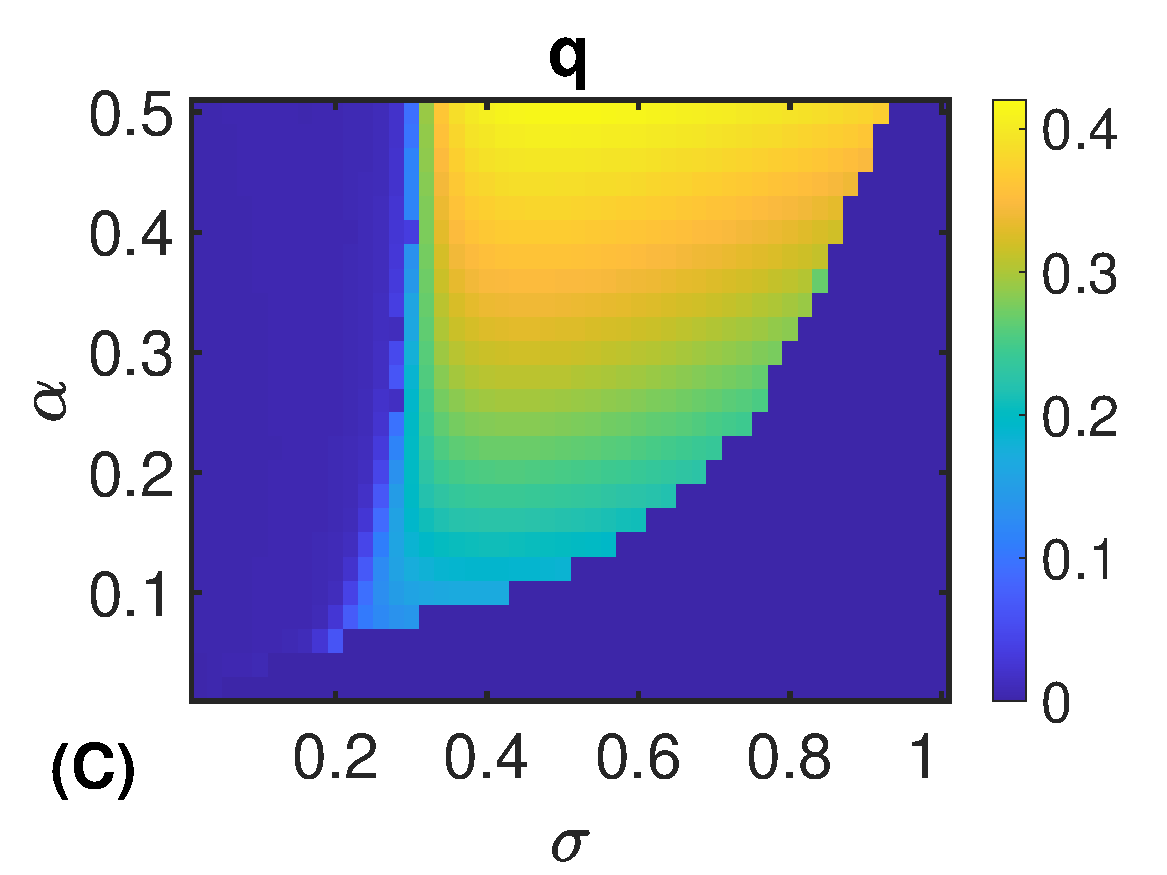
\includegraphics[scale=0.22]{fig1c-eps-converted-to.pdf}

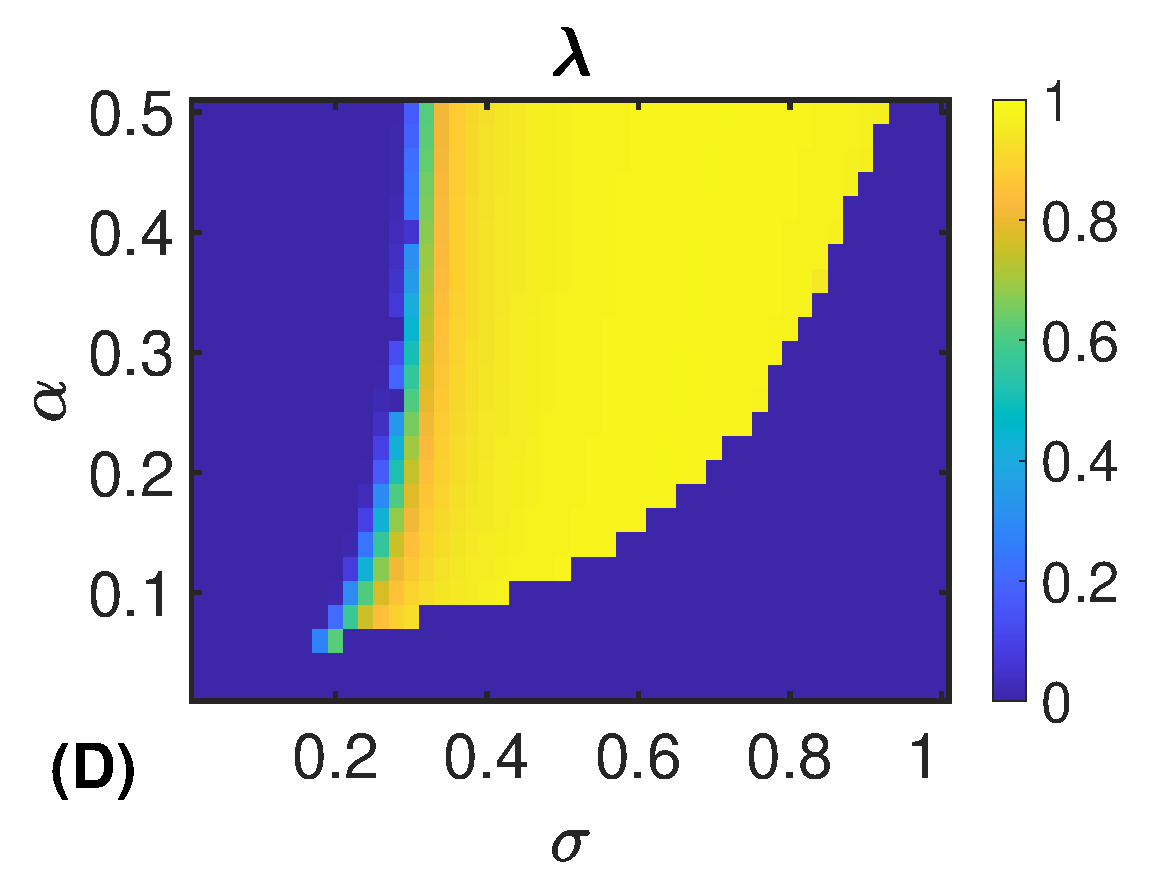
\includegraphics[scale=0.22]{fig1d-eps-converted-to.pdf}
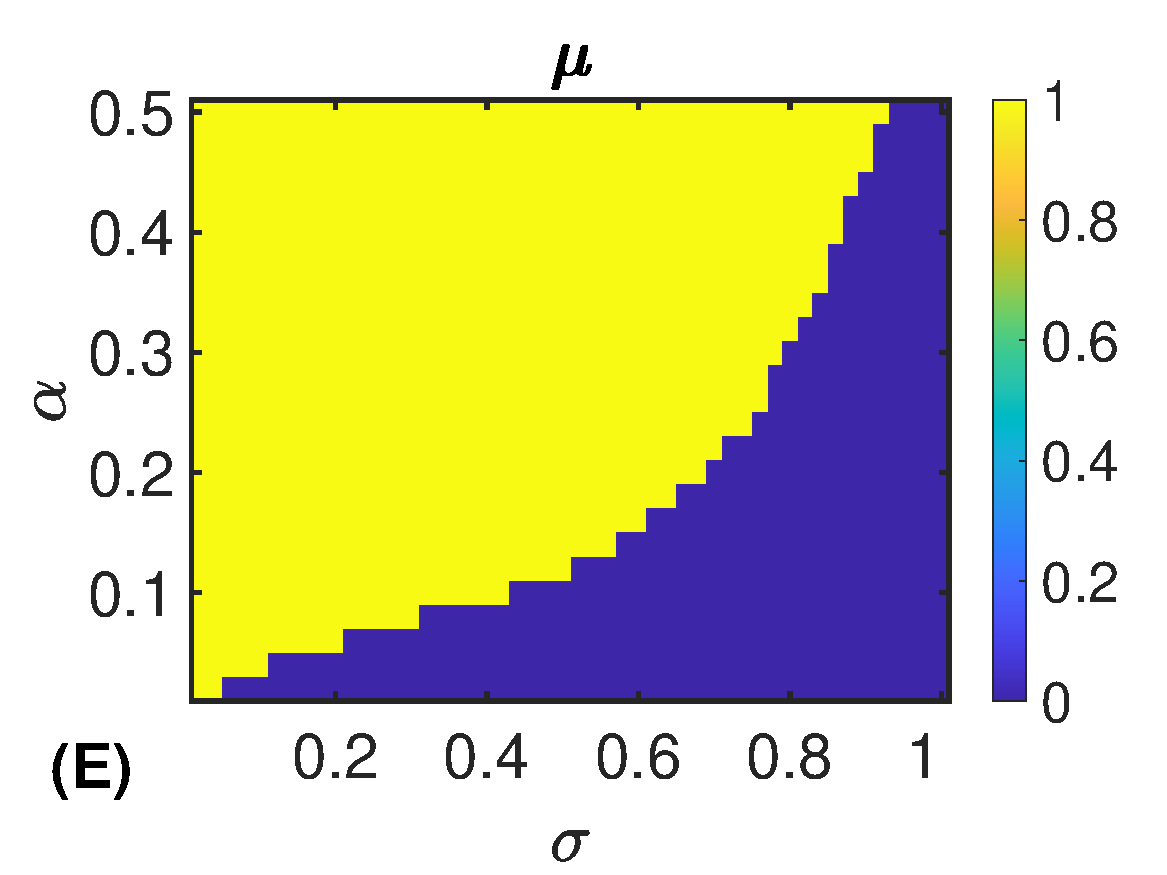
\includegraphics[scale=0.22]{fig1e-eps-converted-to.pdf}
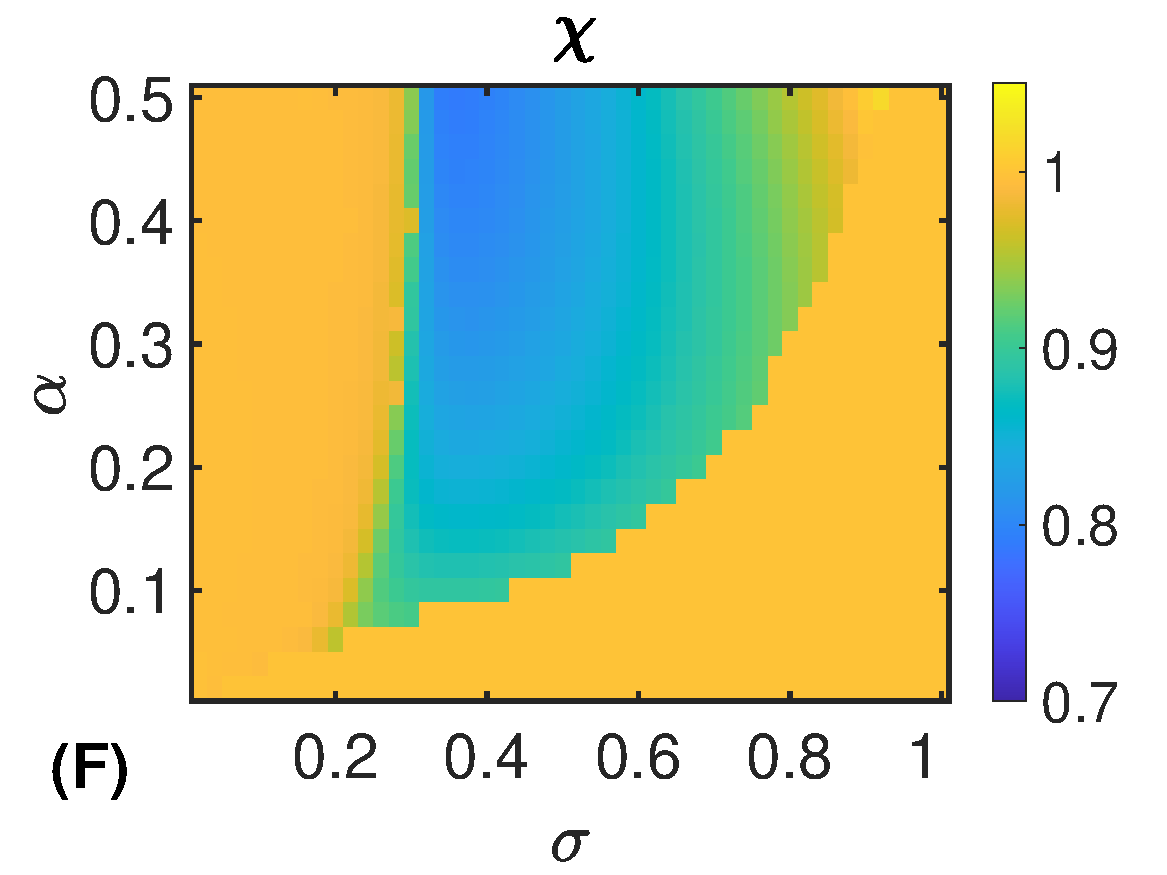
\includegraphics[scale=0.22]{fig1f-eps-converted-to.pdf}
\caption{Order parameters as function of $\alpha = N_o/N_t$ and $\sigma$  at $\beta = 10$. \textbf{(A)}   The model phase diagram. \textbf{(B)} Averaged activity of target genes $m$. \textbf{(C)} The variance in the activity of target genes $q$. \textbf{(D)}  The average of target vs non-target coupling $\lambda$.  \textbf{(E)} The average of target vs target coupling $\mu$. \textbf{(F)} The integrated response  of target spins $\chi$. 
} 
\label{fig:fig3}
\end{figure}


% \begin{figure}[t]
 %\includegraphics[scale=0.8]{evolution_low_noise.png}
%\includegraphics[scale=0.8]{evolution_high_noise.png}

%\includegraphics[scale=0.57]{sampled_traj_low_noise.png}
%\includegraphics[scale=0.57]{sampled_traj_inter_noise.png}
%\includegraphics[scale=0.57]{sampled_traj_para.png}
%\caption{Timeseries of the order parameters at low noise $\sigma = 0.1$ (left column);  intermediate noise $\sigma = 0.8$ (middle column) and high noise $\sigma = 1$ (right column). In all panels,  the vertical red line is to mark the two stages of phenotypic evolution.  Here the timeseries for time $\in [0,30]$ is first generated at $\sigma = 0.8$ and $\sigma = 1$, respectively, then  are continued after time $= 30$ by decreasing the noise level to zero.  In all panels the thick dashed lines denote the mean value of $x$ over $1000$ trajectories.
%} 
%\label{fig:fig3}
%\end{figure}
\end{document}
 \subsection*{B. Closure scheme for stationary state in the zero-noise limit}
We consider $\sigma = 0$. Depending on the realization of $\tilde{z}$, the \emph{random} fixed point $x_*$ can be either zero or non-zero.  Denoting   $x_0 = \mu\cdot m_\infty + J_0^2 \chi  x_* \,+\,J_0\sqrt{q}\tilde{z}$ and $J_0= \lambda \sqrt{\alpha}$, we have,
%\begin{equation}
 %   \left \{ \begin{array}{l} \displaystyle   q := \big \langle x_*^2 \big\rangle = \int_{-\infty}^{\infty} Dz \int_{-\infty}^{\infty} D\tilde{z}  \big[{\rm tanh}(x_0)+ \sigma z \big]^2 \\  \\ \displaystyle   m_\infty := \big \langle x_* \big\rangle = \int_{-\infty}^{\infty}  Dz   \int_{-\infty}^{\infty} D\tilde{z}  \big[{\rm tanh}(x_0)+ \sigma z \big]   \\ \\\displaystyle 
  %\chi = \frac{1}{J_0\sqrt{q} } \int_{-\infty}^{\infty}  Dz  \int_{-\infty}^{\infty}  D\tilde{z} \cdot 
%\frac{\partial x(z, \tilde{z})}{\partial \tilde{z}}\, \, \end{array} \,\right.\,    \,,\quad \frac{\partial x(z, \tilde{z})}{\partial \tilde{z}} = \frac{J_0\sqrt{q} \big(1- f_0^2(\tilde{z})\big)}{\displaystyle 1- J_0^2 \chi \cdot \big(1- f_0^2(\tilde{z})\big)}  \,  \label{order_parameter_from_closed1}
%\end{equation}
 from the linear approximation of $f_0:= {\rm tanh}(x_0)\simeq x_0$ for $x_0 \ll 1$, % yields $x_*(\tilde{z},z) = \mu\cdot m_\infty + J^2_0 \chi \cdot x_* (\tilde{z},z) + J_0 \sqrt{q}\tilde{z}  +  \sigma z $, or equivalently 
\begin{subequations}
\label{allequations11}
 \begin{eqnarray}
x_*(\tilde{z},z)& =& \frac{J_0 \sqrt{q}}{1- J_0^2 \chi}\, \Big(\Delta(z) + \tilde{z} \Big) \,, \qquad \Delta(z) = \frac{\mu \cdot m_\infty + \sigma z}{J_0\sqrt{q}} \label{small_fixed_point}\\ x_*(\tilde{z},z)&>&0\,\quad {\rm and}\,\quad  \partial x_*/\partial \tilde{z} > 0\,\quad {\rm if}\,\quad
\tilde{z} > - \Delta(z) \,\quad {\rm and}\,\quad 1 > J_0^2 \chi
\end{eqnarray}
\end{subequations}
Under the condition that $\mu >0$, using Eq. \eqref{small_fixed_point}, we can rewrite the Eqs. \eqref{closed1} as
\begin{equation}
    \left \{ \begin{array}{l} \displaystyle   \frac{m_\infty}{\sqrt{q}} = \frac{J_0}{\displaystyle  1 -J_0^2 \chi }\,  \cdot\omega_1\,,\qquad  \omega_1 :=  \int_{-\infty}^\infty Dz \int_{-\Delta(z)}^\infty D\tilde{z} \cdot \Big(\Delta(z) + \tilde{z} \Big) \\ \\  1 = \displaystyle \frac{J_0^2}{\displaystyle  \big[1 -J_0^2 \chi \big]^2}\,\cdot \omega_2 \,,\qquad \omega_2 := \int_{-\infty}^\infty Dz \int_{-\Delta(z)}^\infty D\tilde{z} \cdot \Big(\Delta(z) + \tilde{z} \Big)^2 \\ \\ \displaystyle 
  \chi = \frac{\Phi}{\displaystyle  1 -J_0^2 \chi }\,,\qquad \qquad \quad \Phi :=  \omega_0 = \int_{-\infty}^\infty Dz \int_{-\Delta(z)}^\infty D\tilde{z} 
 \end{array} \right.\,   \Leftrightarrow  \left \{ \begin{array}{l}  \displaystyle   \frac{m_\infty}{\sqrt{q}} = \frac{\omega_1}{\sqrt{\omega_2}}    \\ \\ \displaystyle   \chi = \frac{\Phi}{J_0 \sqrt{\omega_2}} \\ \\ \displaystyle   \omega_2 = J_0^2 \cdot \big[\omega_2 + \omega_0 \big]^2
     \end{array} \right.\, 
\label{order_parameter_from_closed1_with_Phi}
\end{equation}
where $\Phi$ is the probability that a given gene attains a non-zero fixed point as $t\rightarrow \infty$.
Note that $\Delta(z)$ is a monotonic increasing function of $z$ that can be identified as the root of the last among these equations. %This root does not depend on both $\mu>0$ and $\sigma$, but only on $\alpha$,  and hence, as a consequence, so do both $\chi$ and  $m_\infty/\sqrt{q}$.

The local stability of such small \emph{non-zero} fixed points can be studied using an ansatz
\begin{equation}
    \left \{ \begin{array}{l} \displaystyle x(t) = x_* +\varepsilon x_1(t)  \\ \\ \displaystyle \eta(t) = J_0\sqrt{q} \tilde{z} +\varepsilon \nu(t)
     \end{array} \right.\, 
     \label{ansatz}
\end{equation} 
for which $x_1(t)$ satisfies an equation
$$   \dot{x}_1 = -x_1 + J_0^2 \int_0^t dt' G(t,t') x_1(t') + \nu(t) +\varepsilon(t)$$
that can be written in the Fourier space as follows
\begin{subequations}
\label{allequations12}
 \begin{eqnarray}
    i\omega \tilde{x}_1(\omega) &=& -\tilde{x}_1(\omega) + J_0^2 \tilde{G}(\omega) \tilde{x}_1(\omega) + \tilde{\nu}(\omega) +\tilde{\varepsilon}(\omega) \\    
    \Big[i\omega +1 -  J_0^2 \tilde{G}(\omega) \Big]\tilde{x}_1(\omega)& = & \tilde{\nu}(\omega) +\tilde{\varepsilon}(\omega)
\end{eqnarray}
\end{subequations}
This will be dominated by the zero mode $\omega = 0$, for which $\tilde{G}(\omega =0 ) =\chi$ and hence
\begin{equation}
   \Big\langle \big|\tilde{x}_1(0) \big|^2\Big\rangle = \Phi \frac{J_0^2 \Big\langle \big|\tilde{x}_1(0) \big|^2\Big\rangle +1}{\big[1 -  J_0^2\chi \big]^2 } 
\end{equation}
The factor $\Phi$ accounts for the fraction of non-zero fixed points as only they contribute to the behaviour of the correlation. From the divergence of $ \Big\langle \big|\tilde{x}_1(0) \big|^2\Big\rangle $, we obtain
\begin{equation}
   \Phi =  \frac{\big[1 -  J_0^2\chi \big]^2 }{J_0^2} = \omega_2
\, \quad \Rightarrow  \chi = \frac{\sqrt{\Phi}}{J_0}  \,,\quad \frac{m}{\sqrt{q}} = \frac{\omega_1}{\sqrt{\Phi}}  \quad {\rm and} \,  \quad  J_0^2  = \frac{1}{4\Phi} \end{equation}
As $  \Phi =  \omega_2$, we find   $\Delta = 0$ and hence $\Phi = 1/2$. %, then, substituting this pair value of values into the set of Eq. \eqref{order_parameter_from_closed1_with_Phi} results in
   %$$m_* = \sqrt{\frac{q}{\pi}} \,,\qquad {\rm for\,\, any}\,\,  \sqrt{\frac{q}{2\pi}} = - \sigma z \Rightarrow z \in (-\infty, -\delta)\,,\qquad \delta = \frac{1}{\sigma}\, \sqrt{\frac{q}{2\pi}} $$

\subsection{C. Memory Onset}
The multiple fixed point solutions can be though of as   bifurcating  from this unique time-translation invariant  fixed point  if assuming that in the presence of memory the retard field term takes the following ansatz
\begin{equation} 
G(t,t') = G_0(t-t') + \epsilon G_1(t,t')\,,\quad \epsilon\ll 1
\end{equation}
Under  this ansatz, and further assuming that $G_1(t,t') = G_1(t')$, i.e., the effect of memory depends only on the starting point $t'$ of a perturbation, then to the first order in $\epsilon$, the original fixed point is perturbed correspondingly into 
\begin{equation}
   \tilde{x}_* = \epsilon  x_1(t) + x_* = {\rm tanh}\left(w_0\cdot m_*   + J_0^2 \chi x_* \,+\,J_0\sqrt{q}\tilde{z}  + \epsilon J_0^2 \int_0^t dt'\,G_1(t')x(t')\right) + \sigma z
\end{equation}
We obtain a Taylor expansion for $$f(x)= {\rm tanh} (x) = f_0 + \sigma z + \epsilon \cdot \left[J_0^2   \int_0^t dt'\,G_1(t')x(t')\right]\frac{df}{dx}|_{x = w_0\cdot m_*  + J_0^2  \chi x_*  \,+\,\,J_0\sqrt{q}\tilde{z} } $$ 
So that
$$ x_1(t) = \big[ 1- f_0^2\big]\times \left[J_0^2   \int_0^t dt'\,G_1(t')x(t')\right]$$
Taking derivatives of both sides wrt a perturbing field $ \delta \tilde{h}(t'')$, we get
$$G_1(t'') :=\delta x_1(t)/\delta \tilde{h}(t'') = \big[ 1- f_0^2\big] J_0^2 \int_0^t dt'\,  \frac{\delta x(t')}{\delta \tilde{h}(t'')} G_1(t')$$
Integrating over $t''$ on both sides, we get
$$\hat{\chi} := \int_0^{t'} dt''\,  G_1(t'') = \big[ 1- f_0^2\big] J_0^2 \chi \cdot \hat{\chi}$$
A non-trivial solution leading to non-ergodic behaviour exists if and only if
\begin{equation}
     \big[ 1- f_0^2\big] J_0^2 \chi =1
\label{divergence_chi}
\end{equation}
Here the onset of the transition from spin-glass like fixed points to the ferro-like fixed point  can be identified with the loss of stability of the former as intensity $\sigma$ decreases. Using the same ansatz as in Eq. \eqref{ansatz}, we obtain
$$\dot{x}_1 = -x_1 + \varepsilon(t)+ \big(1-f_0^2\big)\Big[\nu(t) + J_0^2\int dt' G(t,t') x_1(t')\Big]$$
The Fourier component corresponding to $\omega=0$ reads
$$\Big\langle \big|\tilde{x}_1(0) \big|^2\Big\rangle =  \frac{1}{ \Big[1 - \big(1 - f_0^2\big) J_0^2\chi \Big]^2 - J_0^2 \big(1 - f_0^2\big)}$$
For each of those fixed points, $x_*(z;\sigma)$ its corresponding instability condition becomes 
\begin{equation}
   \Big[1 - \big(1 - f_0^2\big) J_0^2\chi \Big]^2 = J_0^2 \big(1 - f_0^2\big)
   \label{instability}
\end{equation}
where 
$$f_0(x_*) ={\rm tanh}\left(w_0.m_*  + J_0^2\chi  x_*  \,+\,J_0\sqrt{q}\tilde{z} \right) \,,  $$
It is straightforwards to check that as $f_0\rightarrow 1$, Eq \eqref{instability} reduces to the memory onset condition Eq. \eqref{divergence_chi},
in agreement with the result obtained by analysing the effect of long-term memory.
As a result of $f_0\rightarrow 1$, we further have   
$$ x_* = 1 + \sigma z\,, \qquad q = \sigma^2 +1 \,,\qquad m = 1$$
Integrating both sides of Eq. \eqref{instability}, we obtain a similar to AT line condition
\begin{equation}
     0< 1 - \alpha^{-1} (1+ 2\chi) (1+\sigma^2 - q)  + \alpha^{-2} \chi^2 \int Dz (1-f_0)^4 
\end{equation}
       
 


